\chapter{Realizace}
\label{realizace}
% promereni zapojeni jestli vse funguje 
% TODO + struktura firmware a provadeni digitalniho testu -> KAM TO ZARADIT? mozna do subsection realizace?
V této části bude popsána detailní realizace celého zařízení. V předchozích částech byly zmíněny základní požadavky \ref{Technicka specifikace} na návrh celého vyčítacího rozhraní a uveden základní koncept řešení \ref{Koncept reseni}. Při realizaci individuálních částí rozhraní byly tyto požadavky respektovány. Dále jednotlivé části realizace byly vybírány s ohledem na miniaturizaci a celkovou spotřebu vyčítacího rozhraní. 

\par Pro další části textu bude označení desek plošných spojů navrženého rozhraní shodné, s označením schematického návrhu konceptu řešení z obrázku \ref{fig:navrh_reseni}. Cílem řešení bylo co nejvíce funkcionalit rozhraní implementovat na základní desce. Prvním důvodem bylo, že druhá deska plošných spojů, obsahuje detektor Timepix 2, který je v celém návrhu nejdůležitější a nejsložitější částí. Pokud by bylo vše implementováno na jedné desce plošných spojů, při jakémkoliv problému musí být vyměněna celá deska i s detektorem Timepix 2. Při rozložení rozhraní na dvě desky plošných spojů dojde při případném problému k výměně jen základní desky, popřípadě desky s detektorem Timepix 2. 
\par Druhým důvodem rozložení rozhraní na dvě desky plošných spojů je miniaturizace vyčítacího rozhraní. Za použití dvou desek plošných spojů, spojenými konektorem celé rozhraní zvýší své rozměry pouze na výšku o 3 mm přitom rozměry desky s detektorem Timepix 2 mohou být stejné jako desky základní.

\par Realizace návrhu obou desek plošných spojů probíhala v programu Altium Designer. Mechanické integrace rozhraní, především validace případných kolizí plošných spojů s navrženou mechanikou, probíhala v programu Autodesk Inventor. Pokud nebude uvedenou jinak, pořízené obrázky dokumentace řešení jsou z těchto programů.

\section{Základní deska}	
	\label{zakladni deska}
	Základní deska je navržena na šesti vrstvém plošném spoji. Rozložení jednotlivých vrstev lze vidět na obrázku \ref{tab:pcb_vrstvy}. Celková tloušťka navrženého PCB je dle celkové skladby z obrázku \ref{fig:PCB_mother_stackup}, 1.6 mm. Vnější rozměry základní desky jsou 53 x 17 mm. Obecné složení základní desky, je shodné s blokovým konceptem řešení z části \ref{fig:navrh_reseni}. Dále bude popsána detailní struktura jednotlivých částí navržené základní desky.

\begin{figure}
	\begin{minipage}[b]{.45\linewidth}
		\centering
		\captionsetup{justification=centering}
		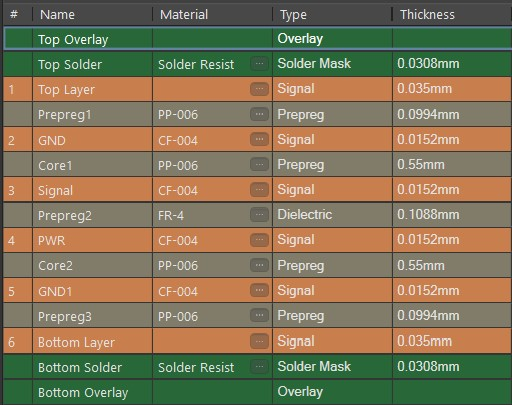
\includegraphics[scale=0.60]{PCB_mother_stackup.jpg}
		\caption{Základní deska. Rozložení vrstev.} 
		\label{fig:PCB_mother_stackup}
	\end{minipage}\hfill
	\begin{minipage}[b]{.45\linewidth}
		\centering
		\begin{tabular}{ |P{3cm}||P{3,5cm}|  }
			\hline
			\multicolumn{2}{|c|}{Popis vrstev základní desky.} \\
			\hline
			Vrstva  & Popis\\ \hline \hline 
			1 - TOP& Signálová vrstva\\ \hline		
			2 - GND1& Zemní vrstva \\ \hline 		 
			3 - SIG& Signálová vrsta \\ \hline
			4 - PWR& Napájecí vrstva\\ \hline
			5 - GND2& Zemní vrstva\\ \hline
			6 - BOT& Signálová vrstva\\ \hline
		\end{tabular}
		\caption{Popis vrstev základní desky.}
		\label{tab:pcb_vrstvy}
	\end{minipage}
\end{figure}

	\subsection{Napájení}
	\label{napajeni}
	Na základní desce je realizováno napájení, které je dále používáno pro celé vyčítací rozhraní. Celkem jsou na základní desce tři spínané synchronní step-down buck regulátory. Konkrétně se jedná o regulátory MP2333H \cite{MPH2333} od společnosti Monolithic Power Systems. Regulátory pracují v rozsahu vstupních napětí on 4.2 V do 18 V. Maximální výstupní proud jsou 3 A a spínací frekvence regulátoru je 1.2 MHz. Regulátory je možné použít v pouzdře SOT583, s rozměry 1.6 x 2 mm, které jsou pro úlohu miniaturizace rozhraní vyhovující. V tabulce \ref{tab:napajeni} je uvedený detailnější popis napájecích úrovní, které jsou generovány na základní desce.
	\begin{table}[h!]
		\centering
		\begin{tabular}{ |P{3cm}||P{10cm}|  }
			\hline
			\multicolumn{2}{|c|}{Napájení základní desky vyčítacího rozhraní} \\
			\hline
			Napájení  & Popis\\ \hline \hline 
			+5V & Externí napájení vyčítacího rozhraní přes USB typu C \\ \hline		
			+3V3 & Napájení pro mikrokontrolér a CPLD \\ \hline 		 
			+2V5 & Napájení vstupní a výstupní brány detektoru Timepix 2 \\ \hline
			+1V2 & Napájení vstupní/výstupní brány CPLD\\ \hline
		\end{tabular}
		\caption{Napájení základní desky vyčítacího rozhraní.}
		\label{tab:napajeni}
	\end{table}
	Napájení uvedené v tabulce \ref{tab:napajeni} jsou až na napájení 1.2 V, dostupné také na druhé desce plošných spojů s detektorem Timepix 2. Více o propojení signálů základní desky a desky s detektorem Timepix 2 lze dohledat v části textu \ref{konektor}. Ukázkové schematické zapojení jednoho ze tří spínaných regulátorů, můžete vidět na obrázku \ref{fig:mp2333h}. Konkrétně se jedná o zapojení, při kterém uvedený regulátor reguluje ze vstupních +5 V na výstupní napájení +1.2 V.
	\begin{figure}[h!]
		\centering
		\captionsetup{justification=centering}
		\includegraphics[scale=0.50]{mp2333h.pdf}
		\caption{Zapojení regulátoru MP2333H.} 
		\label{fig:mp2333h}
	\end{figure}
	\subsubsection{Napájecí sekvence}
	Napájecí sekvenci je možné vidět na zjednodušeném diagramu na obrázku \ref{fig:napajeci_sekvecne}. Po připojení USB typu C do konektoru na základní dece je dostupné napájení +5 V. Těchto +5 V spíná v napájecí sekvenci první regulátor, který generuje na výstupu +3.3 V. Pokud je toto výstupní napájení +3.3 V v pořádku, integrovaný obvod tuto informaci signalizuje pomocí pinu PG. Právě tento pin PG, signál PG\_3V3, může být je připojen na vstupní pin dalšího regulátoru a to na pin regulátoru generující výstupní napětí +2.5 V. V návrhu řešení je možné vybrat mezi uvedeným propojením, nebo je možné regulátor pro napájení +2.5 V možné řídit z mikrokontroléru. Poslední regulátor na základní desce s výstupním napětím +1.2 V je řízený z mikrokontroléru, neboli jeho vstupní pin EN je propojen signálem EN\_1V2 s výstupní bránou mikrokontroléru.
	\begin{figure}[h!]
		\centering
		\captionsetup{justification=centering}
		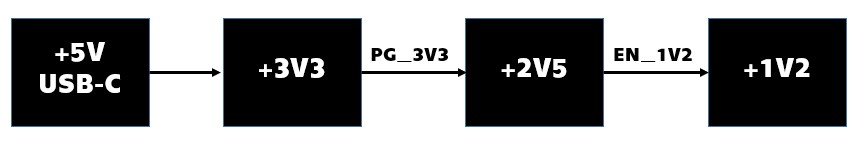
\includegraphics[scale=0.80]{napajeci_sekvence.jpg}
		\caption{Napájecí sekvence základní desky.} 
		\label{fig:napajeci_sekvecne}
	\end{figure}
	\par Výstupní napětí použitého spínaného regulátoru je nastaveno pomocí napěťového děliče ve zpětné vazbě regulátoru a dáno vztahem dle \ref{eq:Vout}. Kde $V_{REF}$ = 805 mV.
	\begin{equation}
		V_{OUT} = \frac{R1 \cdot V_{REF}}{R2} + V_{REF}
		\label{eq:Vout}
	\end{equation}

	\par Z obrázku \ref{fig:napajeci_sekvecne} je vidět, že spínaný stabilizátor generující +3.3 V není programově řiditelný z mikrokontroléru. Spínaný stabilizátor +3.3 V, z mikrokontroléru řídit nelze, protože právě těchto +3.3 V je napájením pro vybraný mikrokontrolér. Možností jakým mimo jiné zajistit dodržení vhodného časování napájecí sekvence základní desky, je propojení PG signálu stabilizátoru +3.3 V na signál EN stabilizátoru +2.5 V, nebo řízením stabilizátoru pro +2.5 V programově z mikrokontroléru. Další možností rozfázování napájecí sekvence je volba vhodného kondenzátoru mezi pinem SS a zemním pinem ze zapojení \ref{fig:mp2333h}. Závislost velikosti výběru kondenzátoru na době rozběhu stabilizátoru je uvedena dle rovnice \ref{eq:Tss}.
	\begin{equation}
		T_{SS}\,[ms] = \frac{2V_{REF} \cdot C_{SS} \,[nF]}{I_{SS}}
		\label{eq:Tss}
	\end{equation}
	Kde $V_{REF}$ = 805 mV a $I_{SS}$ = 7.3 $\mu$A. Ze zapojení \ref{fig:mp2333h} a dosazení do vzorce \ref{eq:Tss} můžeme dopočítat, že náběhový čas spínaného zdroje bude 1.4 ms. Ověření rozfázování napájecí sekvence je uvedeno na obrázku \ref{fig:napajeci_sekvecne_real}. Kde CH1 je napájení +1.2 V, CH2 je +2.5 V a CH3 je vstupních +5V. Při tomto měření byl vstupní pin EN regulátoru pro +2.5 V propojen s výstupním pinem PG, regulátoru s výstupním napětím +3.3 V. Na nastavených kurzorech je také vidět, že teoreticky vypočítaný čas, doby rozběhu regulátoru z rovnice \ref{eq:Tss}, souhlasí s prakticky naměřenými hodnoty. 
	\begin{figure}[h!]
		\centering
		\captionsetup{justification=centering}
		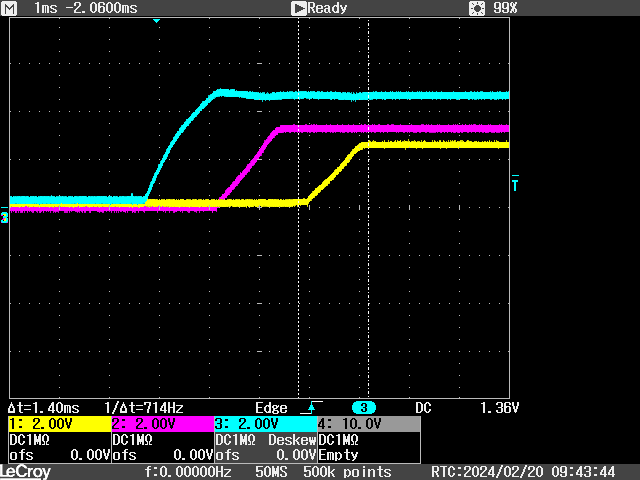
\includegraphics[scale=0.50]{napajeci_sekvence_real.png}
		\caption{Měření napájecí sekvence základní desky.} 
		\label{fig:napajeci_sekvecne_real}
	\end{figure}
	\par Zajištění ochrany, především před elektrostatickým výbojem vstupního napájení, bude popsána v části \ref{USB}. Pouze ve shrnutí, pokud dojde k jakýmkoliv podmínkám, které by mohli elektrostaticky ohrozit vyčítací rozhraní, obvody z části \ref{USB} zajistí vypnutí externího napájení pomocí externího tranzistoru. 

	\subsection{Mikrokontrolér}
	\label{mikrokontolér}
	Pro tuto práci byl vybrán mikrokontrolér od firmy STMicroelectronics, přesněji mikrokontrolér s označením STM32U5A9NJH6Q \cite{STM32U5A9}. Právě tento mikrokontrolér byl vybrán s ohledem na požadavky vyčítacího rozhraní, které byly uvedeny v předchozích částech textu. V následující části budou uvedeny nejdůležitější parametry vybraného mikrokontroléru:
	%\vspace{-5mm}
	\begin{itemize}
		\setlength\itemsep{0.005em}
		\item Jádro : Arm 32-bit Cortex-M33 s DSP a FPU. Frekvence 160 MHz
		\item Napájení 1.7 - 3.6 V
		\item Spotřeba 18.5 $\mu$A/MHz
		\item 4-Mbyte flash s kontrolou EEC
		\item 2514-Kbyte RAM, 66 Kbytes s EEC
		\item 25 Komunikačních periférií
		\item 156 konfigurovatelných vstupních/výstupních pinů
		\item 1x USB OTG High-speed s vestavým PHY 
		\item Pouzdro : TFBGA216. 13 x 13 mm, 0.8 mm mezi pájecími plošky
	\end{itemize}
	\par Prvním požadavkem na mikrokontrolér bylo, aby bylo možné komunikovat s detektorem Timepix 2. V již popsané části textu \ref{Komunikacni rozhrani}, bylo zmíněno, že Timepix 2, dokáže komunikovat přes sériové rozhraní s maximální frekvencí 100 Mhz. Výše uvedený vybraný mikrokontrolér umožňuje konfiguraci sériového komunikačního rozhraní, konkrétněji specifikace SPI až do frekvence 160 MHz. 
	\par Dalším důležitým parametrem při výběru mikrokontroléru byla velikost paměti. Pro vyčtení celé matice pixelů z detektoru Timepix 2, dle \ref{Digitálni cast} vyplývá, že je zapotřebí vyčíst 28 x 256 x 256 bitů dat, tedy 229.376 kB. Výše vybrané parametry pamětí mikrokontroléru jsou pro tento datový tok dostačující.
	\par Nejméně důležitým parametrem při výběru mikrokontroléru byl parametr integrovaného USB přímo uvnitř mikrokontroléru. Neboli není zapotřebí při návrhu USB umísťovat další externí součástky pro implementaci USB komunikace. Tímto parametrem mikrokontroléru bylo dosaženo snížení počtu použitých součástek a tím i zmenšené rozměry celého vyčítacího rozhraní.
	
	\subsubsection{Konfigurace mikrokontroléru}
	Pro práci s mikrokontrolérem jsem použil vývojové prostředí STM32CubeIDE dodávané od společnosti STMicroelectronics, která je výrobcem vybraného mikrokontroléru. Výhodou vývojového prostředí je přímočará grafická konfigurace celého mikrokontroléru s kombinací s klasickou programovou konfigurací. Na obrázku \ref{fig:STM32CubeIde} můžete vidět příklad nakonfigurovaného mikrokotroléru STM32U5A9 v pouzdře TFBGA216. Tmavě zelené body mezi piny znamenají uživatelsky nastavené rozhraní daného pinů mikrokontroléru. 
	\begin{figure}[h!]
		\begin{subfigure}{0.5\textwidth}
			\centering
			\captionsetup{justification=centering}
			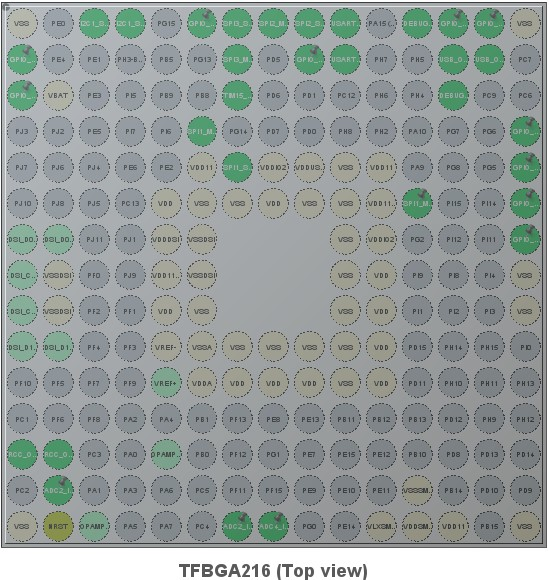
\includegraphics[scale=0.58]{STM32CubeIde.jpg}
			\caption{STM32CubeIDE grafické konfigurace mikrokontroléru.} 
			\label{fig:STM32CubeIde}
		\end{subfigure}
		\begin{subfigure}{0.5\textwidth}
				\centering
			\captionsetup{justification=centering}
			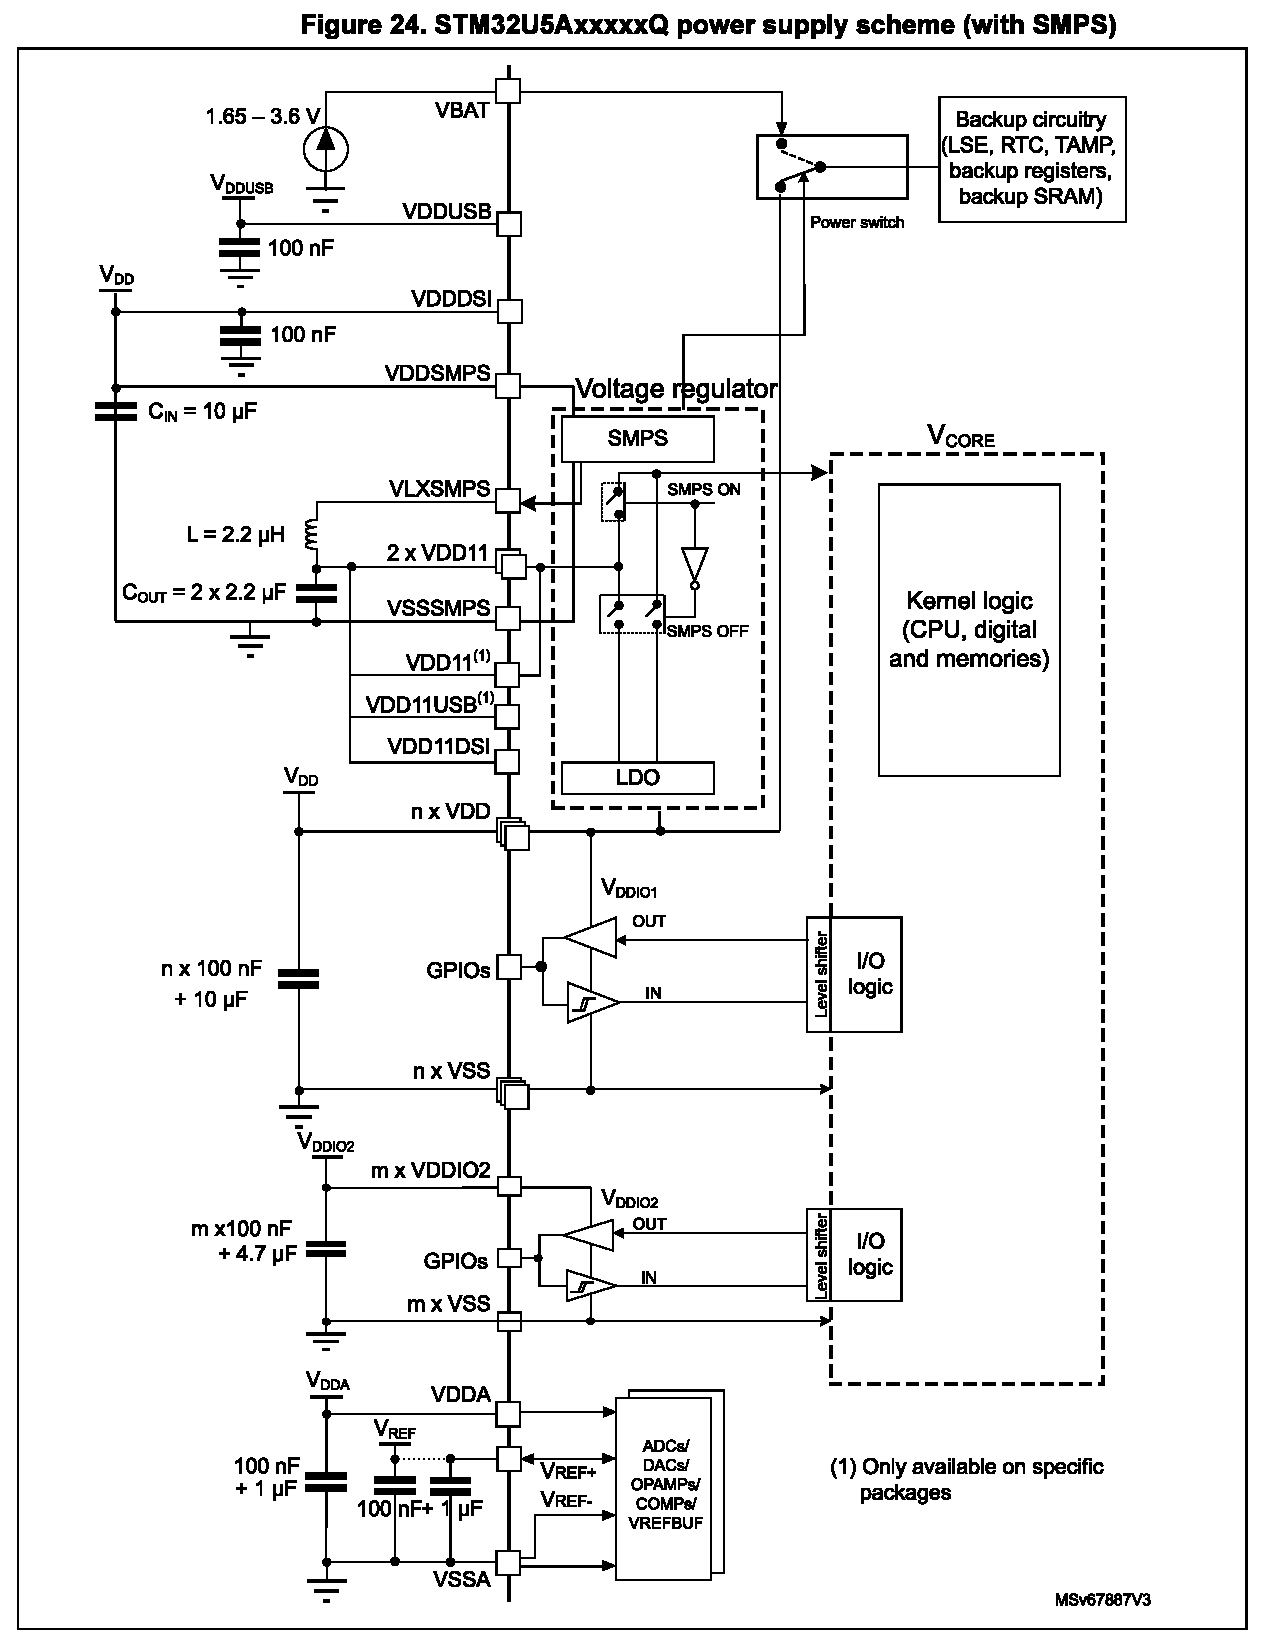
\includegraphics[scale=0.38]{stm32u5_pwr.pdf}
			\caption{Blokové schéma napájení mikrokontroléru.} 
			\label{fig:napajeni_stm32}
		\end{subfigure}
		\caption{Konfigurace a napájení mikrokontroléru STM32U5A9.}
		\label{fig:konfig}
	\end{figure} 
	\begin{table}[h!]
		\centering
		\begin{tabular}{ |P{3cm}||P{10cm}|  }
			\hline
			\multicolumn{2}{|c|}{Napájení potřebné pro mikrokotrolér STM32U5A9} \\
			\hline
			Napájení  & Popis\\ \hline \hline 
			VBAT & Napájení z externí baterie 1.65 - 3.6 V\\ \hline		
			VDDUSB & Napájení pro periférii USB\\ \hline 		 
			VDDSI & Napájení pro periférii DSI \\ \hline
			VDDSMPS & Napájení pro integrovaný spínaný stabilizátor\\ \hline
			VLXSMPS & Spínaný výstup integrovaného stabilizátoru \\ \hline
			VDD11 & Napájení digitální části mikrokontroléru \\ \hline 
			VDD11, VDD & Napájení digitální části mikrokontroléru ze spínaného stab.\\ \hline
			VDDIO2 & Napájení samostatné vstupní/výstupní brány \\ \hline
			VDDA & Napájení analogové části mikrokotroléru \\ \hline
		\end{tabular}
		\caption{Napájení mikrokontroléru STM32U5A9.}
		\label{tab:napajeni_stm32}
	\end{table}
	\subsubsection{Napájení}
	Na obrázku \ref{fig:napajeni_stm32} můžete vidět potřebná napájení pro vybraný mikrokontrolér. 
	Výhodou vybraného mikrokontroléru je, že pro napájení jádra a digitálních periferií využívá spínaného regulátoru, integrovaného přímo na čipu, který je efektivnější v porovnání s lineárním regulátorem. Nevýhodou tohoto napájení je požadavek připojení externí cívky, která je nezbytná pro provoz interního spínaného stabilizátoru a tím i větší požadavky na rozměry celého zapojení. Více podrobností ohledně napájení mikrokontroléru lze najít v referenčním manuálu viz. \cite{STM32U5A9_RM}. Celá realizace schematického zapojení napájení mikrokontroléru je uvedena v přiložené příloze \ref{Priloha základní deska}.
	
	\subsubsection{Konfigurace hodinových signálů} %Pro USB HS plus konfigurace ostatnich periferii ?
	Hodinovým signálem pro jádro mikrokontroléru, který je označován jako SYSCLK, může být jeden ze čtyř dostupných zdrojů hodinového signálu, kterými jsou:
	\begin{itemize}
		\setlength\itemsep{0.005em}
		\item HSE : Externí krystal s parametry frekvence signálu od 4 MHz do 50 Mhz
		\item HSI : 16 MHz interní RC oscilátor 
		\item MSI : Interní RC oscilátor s programově nastavitelnou frekvencí od 100 kHz do 48 MHz
		\item PLL : Fázový závěs, který může mít vstup jeden ze 3 výše uvedených zdrojů hodinových signálů
	\end{itemize}
	Pro realizaci vyčítacího rozhraní byl jako zdroj hodinového signálu vybrán výstup z fázového závěsu, který ze vstupního hodinového signálu HSI generuje hodinový signál o frekvenci 160 MHz. Tento hodinový signál je použit jako zdroj hodinového signálu pro jádro mikrokontroléru a také pro komunikační rozhraní, až na komunikační rozhraní USB. Více informací o konfiguraci hodinového signálu pro USB periferii bude v části \ref{USB}. Samotnou konfiguraci hodinového signálu pro jádro procesoru s využitím fázového závěsu, lze najít na obrázku \ref{fig:hodinovy_signal}
	\begin{figure}[h!]
		\centering
		\captionsetup{justification=centering}
		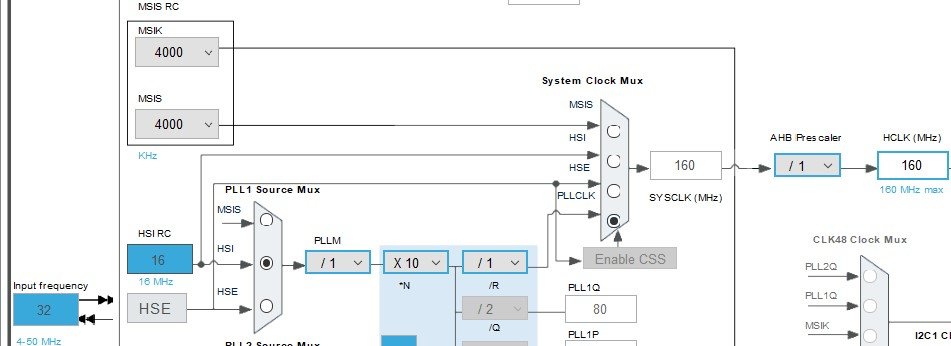
\includegraphics[scale=0.65]{hodinovy_signal.jpg}
		\caption{Konfigurace hodinového signálu pro jádro mikrokontroléru.} 
		\label{fig:hodinovy_signal}
	\end{figure}

	\subsubsection{Periférie SPI}
	Celkem pro implementaci vyčítacího rozhraní byly použity tři SPI periférie:
	 \begin{itemize}
	 	\setlength\itemsep{0.005em}
	 	\item SPI1 : Obecná SPI periférie pro komunikaci se senzory, mimo Timepix 2
	 	\item SPI2 : Použita ke komunikaci s Timepix 2. V konfigurace Master. 
	 	\item SPI3 : Použita ke komunikaci s Timepix 2. V konfigurace Slave.
	 \end{itemize}
 	Periférie SPI1 je nakonfigurována v módu Full-Duplex Master, neboli po sběrnici je možné data z mikrokontroléru odesílat i přijímat. K určení jaké zařízení, připojené na sběrnice SPI1, budou komunikovat slouží signály chip select v realizaci označovány jako nCS (pozn.: prefix n, značí, že signál je aktivní v logické nule). 
 	\par Pro komunikaci s Timepix 2 pomocí sériového rozhraní, byly zvoleny dvě periférie SPI. Popis signálů pro sběrnice SPI2 a SPI3 můžete vidět na obrázku \ref{fig:SPI}. Jak lze ze zapojení vidět, pro komunikace bylo využito celkem 6 signálů. Základní napěťové úrovně, které mají být na signálech v klidovém stavu, jsou určeny pull down, respektive pull up rezistory. 
 	\par Sběrnice SPI2 je nakonfigurována jako Half-Duplex Master. Pomocí této sběrnice se odesílají data do detektoru Timepix 2. Dalšími důležitými parametry nastavení SPI sběrnice je její časování, které musí odpovídat technické specifikaci detektoru Timepix 2. S odkazem na tuto specifikaci \cite{Timepix2}, byla periferie SPI2 nastavena dle \cite{SPI} do módu 3. Neboli pro typ Half-Duplex Master to znamená, že data jsou vysílaná na sestupnou hranu hodinového signálu, přičemž klidový stav hodinového signálu je v logické jedničce.
 	\par Sběrnice SPI3 je nakonfigurována jako typ Half-Duplex Slave. Pomocí této sběrnice se přijímají data z detektoru Timepix 2. Dle \cite{Timepix2} byla sběrnice nakonfigurována do módu 1 \cite{SPI}. Příchozí data z detektoru Timepix 2 jsou vzorkována na sestupnou hranu hodinového signálu, který je společně s daty generován detektorem Timepix 2. Klidový stav hodinového signálu je poté v logické nule.
	\begin{figure}[h!]
 		\centering
 		\captionsetup{justification=centering}
 		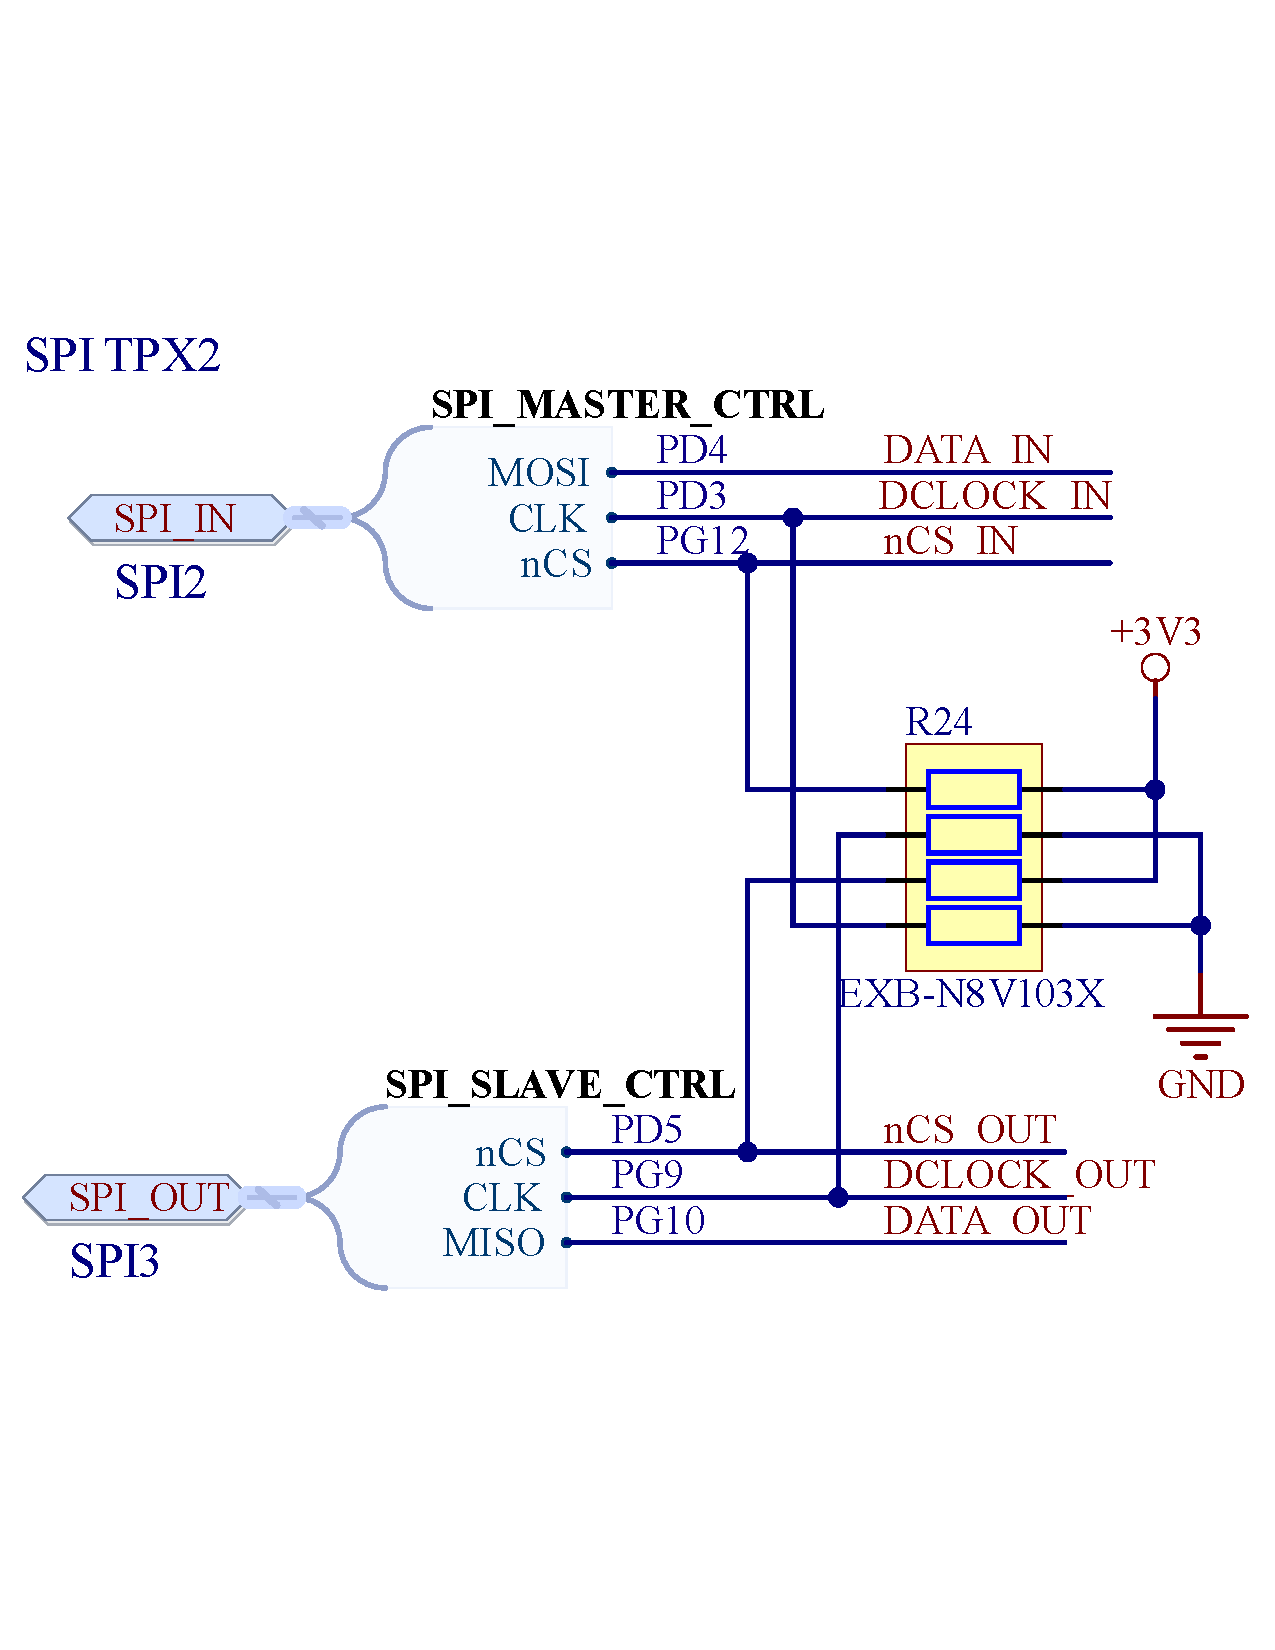
\includegraphics[scale=0.40]{SPI.pdf}
 		\caption{Popis signálů periférií SPI, sloužící pro komunikaci s Timepix 2} 
 		\label{fig:SPI}
 	\end{figure}
 	
 	\subsubsection{Periférie I2C}
 	Další sběrnicí, použitou na vyčítacím rozhraním je sběrnice I2C. Pro celé rozhraní byla použita právě jedna I2C periférie. Pomocí této sběrnice mikrokontrolér monitoruje teplotu na druhé desce plošného spoje s detektorem Timepix 2. Více o komunikaci s teplotním senzorem viz. \ref{Mereni teploty}. Pokud by na I2C sběrnici bylo připojeno více zařízení, určení toho, které zařízení bude po sběrnici komunikovat závisí na fyzické adrese připojeného zařízení. V tomto případě musí být zajištěno, že na sběrnici neexistují dvě zařízení se stejnou fyzickou adresou, jinak by došlo ke konfliktu. 
 	
 	\subsubsection{Periférie UART}
 	\par Periférie UART umožňuje monitorovat průběh programu, který je nahrán do mikrokontroléru, za použití výpisu sériové linky, do příkazové řádky. Signály UART sběrnice jsou vyvedeny na programovací konektor. Popsání programovacího konektoru bude uvedeno následně.

%TODO zminit literaturu ZAHLAVA A MCU
	\subsubsection{Programování}
	Mikrokontrolér je programován pomocí JTAG programovacího rozhraní za využití programovacího konektoru, který je umístěn na spodní straně základní desky \ref{fig:programator}. Jedná se o 12 pinový konektor pro připojení plochého kabelu. Na programování mikrokontroléru byly z mikrokontroléru vyvedeny signály: JTMS/SWDIO a JTCK/SWCLK. Zbylé piny konektoru byly využity pro programování CPLD MachXO2 \cite{CPLD}. Přes plochý konektor z obrázku \ref{fig:programator} lze programovat, jak mikrokontrolér, tak na základní dece použité CPLD MachXO2 \ref{CPLD}. Posledními signály, které byly vyvedeny na programovací konektor jsou signály, pro monitorování běhu programu v mikrokontroléru. Jedná se o signály komunikačního rozhraní sběrnice UART. Signály jsou za pomocí plochého kabelu vyvedeny na redukční desku z obrázku \ref{fig:programator}, na které je možné pomocí propojovacích kabelů připojit programátor ST-Link, kterým je možné použitý mikrokontrolér naprogramovat. 
\begin{figure}[h!]
	\begin{subfigure}{0.5\textwidth}
		\centering
		\captionsetup{justification=centering}
		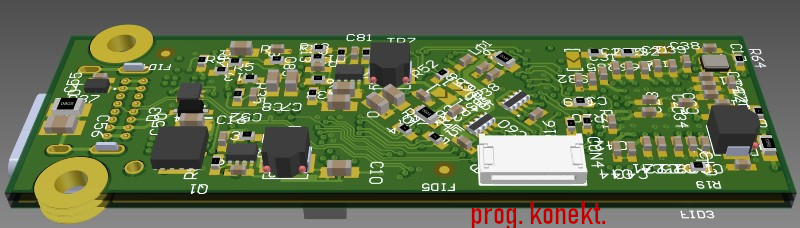
\includegraphics[scale=0.48]{programator.jpg}
		\caption{Programovací konektor.} 
		\label{fig:programator}
	\end{subfigure}
	\begin{subfigure}{0.5\textwidth}
		\centering
		\captionsetup{justification=centering}
		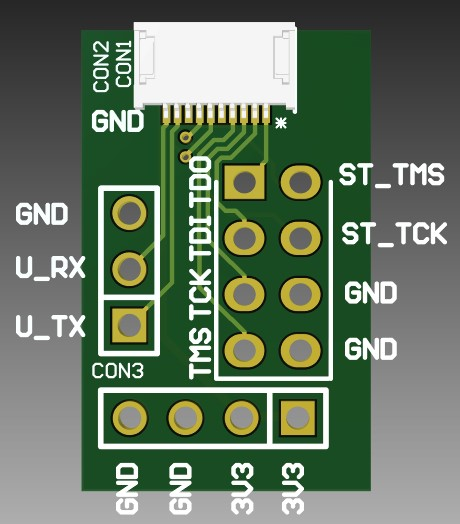
\includegraphics[scale=0.22]{konverzni_deska.jpg}
		\caption{Konverzní deska pro připojení programátoru.} 
		\label{fig:konverzni_deska}
	\end{subfigure}
	\caption{Programování mikrokontroléru.}
	\label{fig:programovani}
\end{figure} 

	\subsubsection{PCB}
	Realizované PCB pro část mikrokontroléru můžete vidět na obrázku \ref{fig:ST_layout}. Na obrázku nejsou uvedeny 3 tři vrstvy PCB, kterými jsou 2., 3. a 5. vrstva. Vrstva 2 a 5 tvoří pod částí mikrokontroléru souvislou zemní plochu a vrstva 3 slouží jako vrstva signálová. Blokovací kondenzátory napájení mikrokotroléru, jsou dle specifikace \cite{STM32U5A9_RM} umístěny co nejblíže příslušným pinům, z druhé strany PCB, než je samotný mikrokontrolér. Toto zapojení je možné vidět na obrázku \ref{fig:ST_BOT}. 
	\begin{figure}[h!]
		\centering
		\captionsetup{justification=centering}
		\begin{subfigure}[b]{0.3\textwidth}
			\centering
			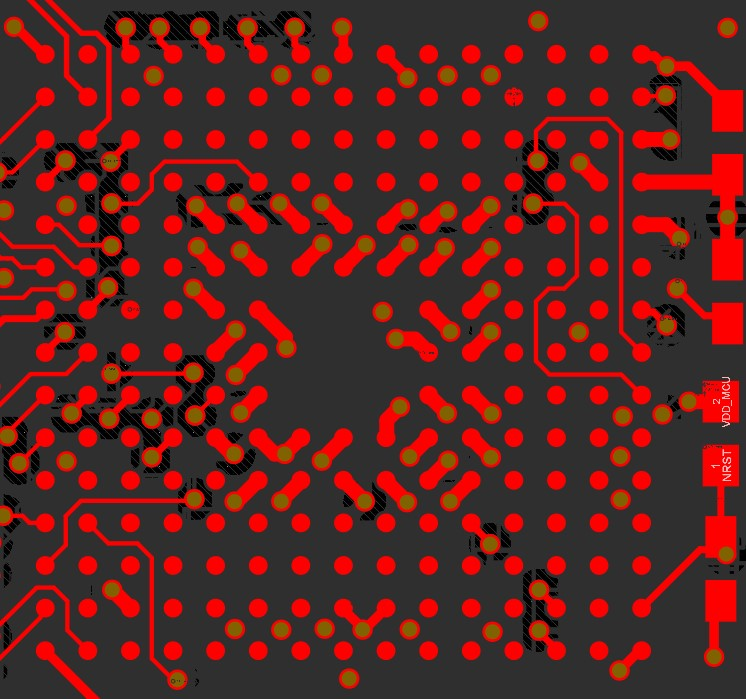
\includegraphics[scale=0.30]{ST_TOP.jpg}
			\caption{Vrchní vrstva PCB STM32U5A9.}
			\label{fig:ST_TOP}
		\end{subfigure}
		\hfill
		\begin{subfigure}[b]{0.3\textwidth}
			\centering
				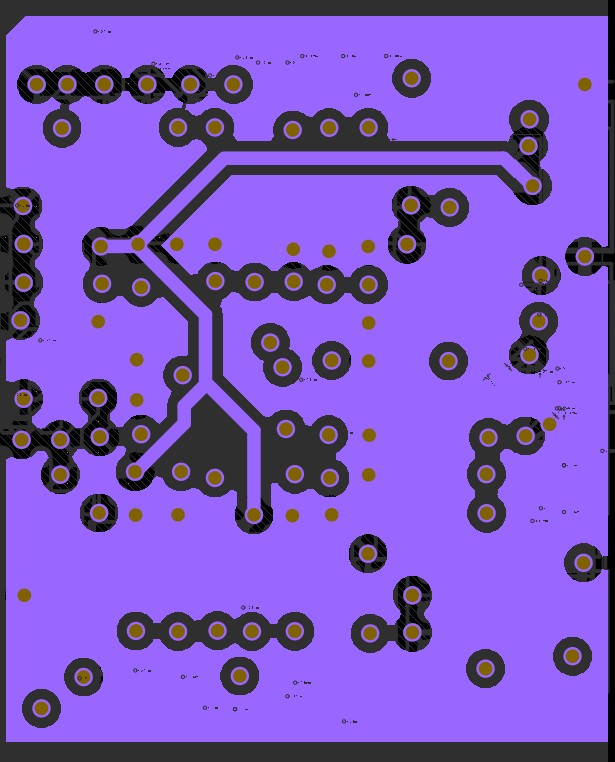
\includegraphics[scale=0.30]{ST_PWR.jpg}
			\caption{Prostřední vrstva PCB STM32U5A9.}
			\label{fig:ST_PWR}
		\end{subfigure}
		\hfill
		\begin{subfigure}[b]{0.3\textwidth}
			\centering
				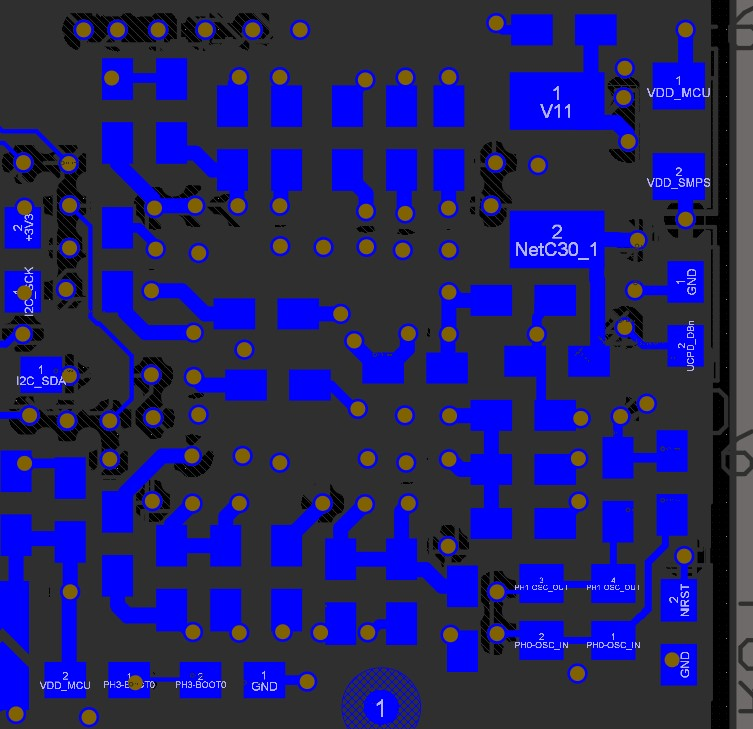
\includegraphics[scale=0.30]{ST_BOT.jpg}
			\caption{Spodní vrstva PCB STM32U5A9.}
			\label{fig:ST_BOT}
		\end{subfigure}
		\caption{STM32U5A9 PCB realizace.}
		\label{fig:ST_layout}
	\end{figure}
	Rozteč mezi jednotlivými piny mikrokontroléru je 0.8 mm. Jak lze vidět na obrázku \ref{fig:ST_TOP}, mezi pájecími plošky jsou umístěny prokovy, kde vnitřní průměr prokovů je 0.3 mm a vnější rozměr 0.4 mm. Prokovy jsou kvůli zvolenému pouzdru BGA mikrokontroléru zamaskované a vyplněné epoxidem, aby při procesu pájení nedošlo ke zkratování prokovů s piny mikrokontroléru.
	\par Osazení mikrokontroléru proběhlo na půdě ČVUT v laboratoři LVR (Laboratoř pro Vývoj a Realizaci). Pro osazení byla použita rework stanice: ERSA - IRPL650A.
	
	\subsection{CPLD}	% CPLDcko - delice, urovne. Odporove site
	\label{CPLD}
	Další hlavní součástí základní desky, je CPLD. Pro tuto práci bylo vybráno CPLD od společnosti Lattice Semiconductor s označením MachXO2 \cite{CPLD}. Jak bude popsáno v následné části, CPLD je použito v této práci pro konverzi logických úrovní a generování diferenciálních signálů, které jsou potřebné pro komunikaci s detektorem Timepix 2. S ohledem na tyto požadavky a miniaturizaci rozhraní bylo vybráno právě CPLD MachXO2 v pouzdře QFN-48. 
	\par Další nabízenou variantou převodu logických úrovní bylo použití vysílače a přijímače LVDS napěťových úrovní. Nevýhodou použití tohoto zapojení je plocha potřebná pro zapojení součástek na desce plošných spojů v důsledku velikosti pouzder vysílače a přijímače LVDS komunikace. Další nevýhodou je výsledná spotřeba zapojení. Jak bylo popsáno v \ref{Komunikacni rozhrani}, potřebné logické úrovně pro Timepix 2 jsou nižší než úrovně LVDS specifikace, tedy bylo by nutné generované úrovně LVDS vysílače upravit na požadovanou úroveň specifikace SLVS. Tato úprava pomocí zapojení odporů je ovšem energeticky neúsporná. Proto bylo zvoleno zapojení se součástkou MachXO2. 
	Programování CPLD probíhalo v prostředí Lattice Diamond.
	
	\subsubsection{Napájení}
	V tabulce \ref{tab:napajni_cpld} můžete vidět napájecí úrovně pro použité CPLD MachXO2. Pro napájení jádra CPLD a vstupních/výstupních bran 0, 1 a 2 bylo použito napájení +3.3 V. Pro vstupní/výstupní bránu 3, je napájecí napětí +1.2 V. Toto napájení bylo zvoleno s ohledem na použití této brány jako typ LVCMOS12D, které slouží pro generování diferenciálních páru odpovídající specifikaci SLVS \ref{fig:SLVS_LVDS}.
	\begin{table}[h!]
		\centering
		\begin{tabular}{ |P{3cm}||P{5cm}||P{3cm}|  }
				\hline
			\multicolumn{3}{|c|}{Napájení CPLD MachXO2} \\
			\hline
			Napájení  & Popis & Hodnota [V]\\ \hline \hline 
			VCC & Hlavní napájení jádra CPLD & +3.3 V\\ \hline		
			VCCIO0, 1, 2 & Napájení brány 0, 1, 2 & +3.3V\\ \hline 		 
			VCCIO3 & Napájení brány 3 & +1.2 V \\ \hline
		\end{tabular}
		\caption{Napájení CPLD MachXO2.}
		\label{tab:napajni_cpld}
	\end{table}


	\subsubsection{Konverze logických úrovní}
	\label{CPLD konverze}
	Dle \ref{Komunikacni rozhrani}, je zapotřebí pro komunikaci s Timepix 2 při využití sériového rozhraní použít komunikační specifikaci typu SLVS \ref{fig:SLVS_LVDS}, využívající diferenciální páry. Použitý mikrokontrolér \ref{mikrokontolér}, je kompatibilní pouze s CMOS 3.3 V logikou. CPLD umožňuje převod těchto úrovní. Respektive převod CMOS 3.3 V logiky na SLVS specifikaci a opačně.
	\par Použité CPLD umožňuje generovat pouze signály ze specifikace Sub-LVDS. Aby bylo dosaženo parametrů potřebných pro SLVS specifikaci, bylo pro každý generovaný výstupní diferenciální pár použito zapojení s odpory z pravé části obrázku \ref{fig:sub_lvds_slvs}. Pro vstupní diferenciální páry, byla pouze co nejblíže k CPLD umístěna terminace, viz. levá část obrázku \ref{fig:sub_lvds_slvs}.
	% TODO davat sem?
\begin{comment} 
	Programová implementace generování diferenciálních signálů pro MachXO2 obsahující pouze část architektury pro konverzi logických úrovní je zobrazena v ukázkovém kódu \ref{kod_vhdl}.
\begin{lstlisting}[frame=single, language=VHDL, caption={Ukázkový kód ve VHDL pro CPLD}, label=kod_vhdl]
	architecture behavioral of t2m is
	begin
	-- CMOS -> SLVS
	DATA_IN_SLVS	<= DATA_IN;
	nCS_IN_SLVS	<= nCS_IN;
	DCLOCK_IN_SLVS	<= DCLOCK_IN;
	MCLOCK_SLVS	<= MCLOCK;
	-- SLVS -> CMOS
	DATA_OUT	<= DATA_OUT_SLVS;
	DCLOCK_OUT	<= DCLOCK_OUT_SLVS;
	nCS_OUT		<= nCS_OUT_SLVS;
	end architecture behavioral ;
\end{lstlisting}
\end{comment}
	
	\begin{figure}[h!]
	\centering
	\captionsetup{justification=centering}
	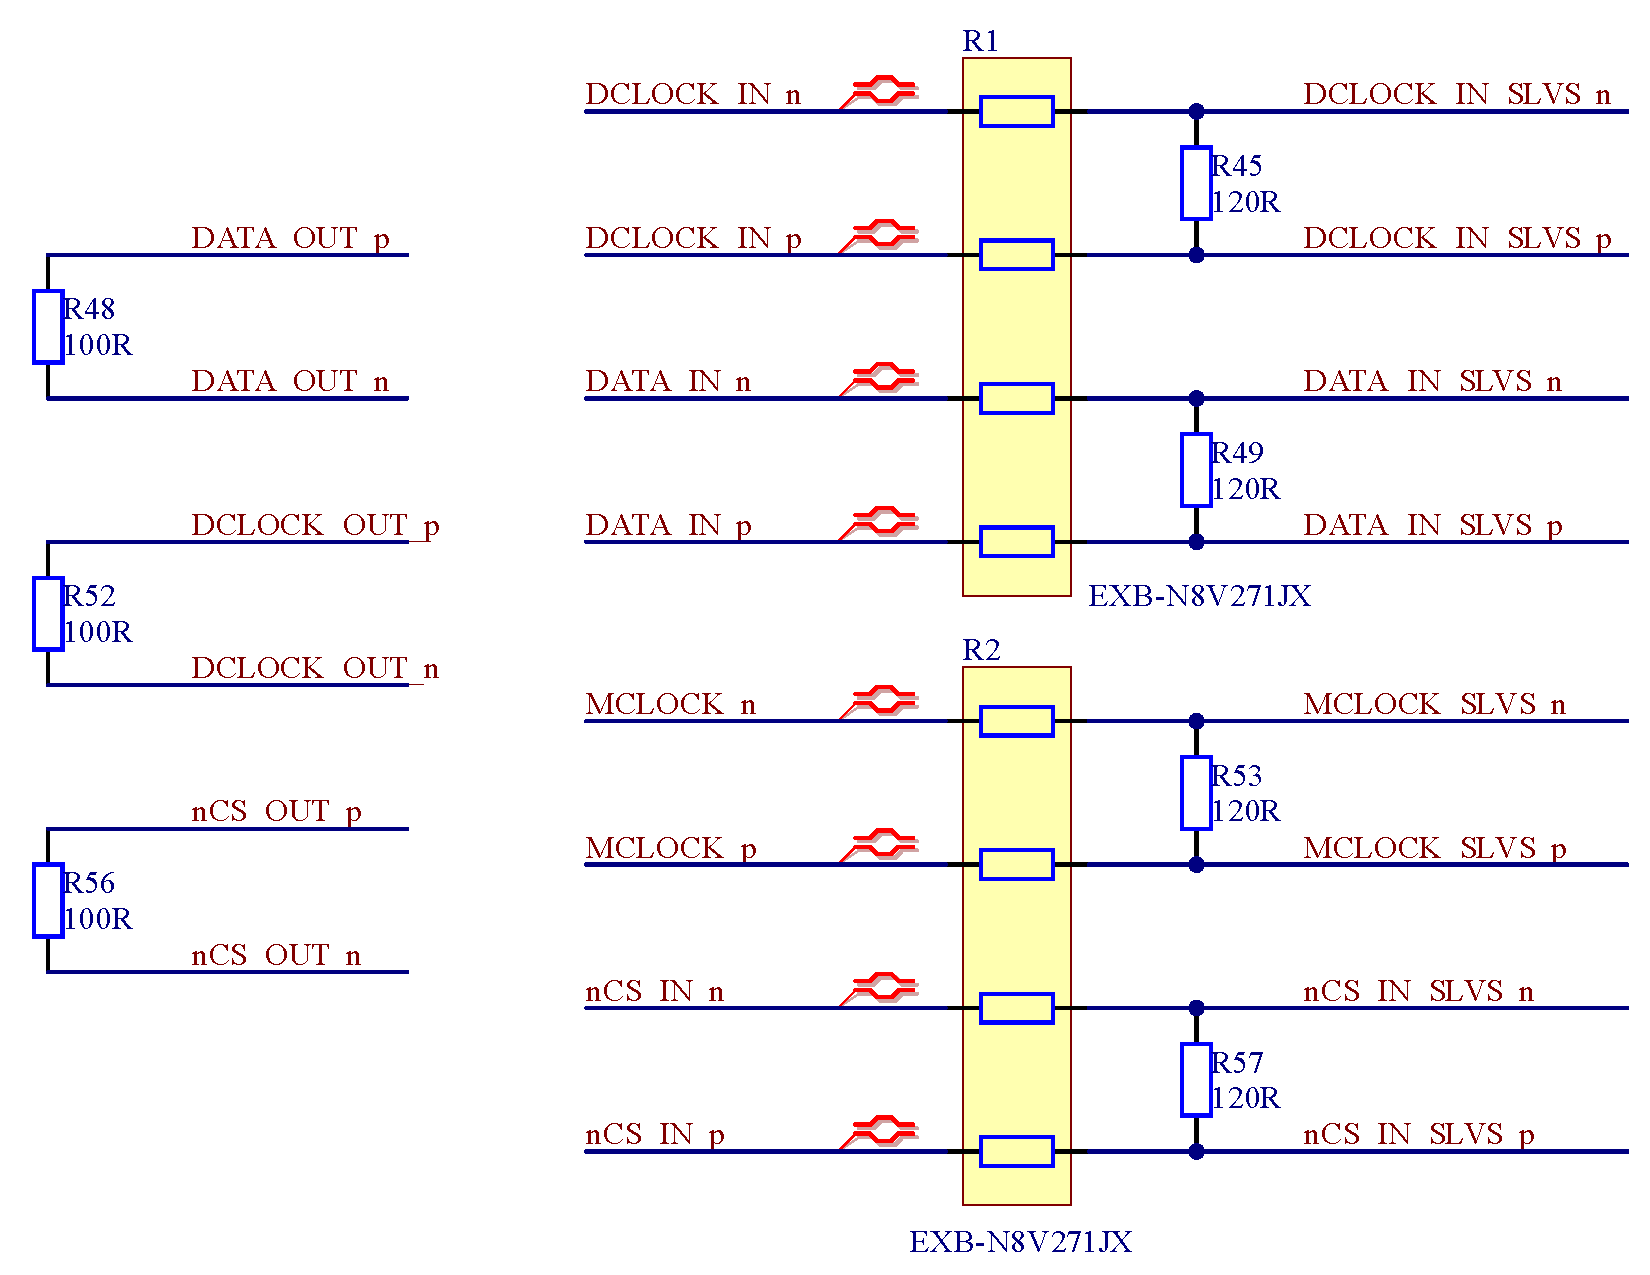
\includegraphics[scale=0.50]{sub_lvds_slvs.pdf}
	\caption{Konverze napěťových úrovní standartu Sub-LVDS na SLVS.} 
	\label{fig:sub_lvds_slvs}
	\end{figure}
	\subsubsection{Programování}
	Pro programování CPLD byly zvoleny dvě možnosti. Primární možností je programování CPLD, přes externí programovací konektor, který se používá pro programování mikrokontroléru \ref{fig:programator}. Na tento konektor jsou vyvedeny signály: TDO, TDI, TMS a TCK z CPLD. Druhou možností je programování CPLD pomocí mikrokontroléru za využití SPI sběrnice. Výhodou možnosti programování CPLD z mikrokontroléru je možnost měnit konfiguraci CPLD za běhu programu mikrokontroléru. V této práci je tato možnost pouze připravena pro případné budoucí využití. S ohledem na využití CPLD, jako překladače napěťových úrovní, není zapotřebí jakkoliv konfigurovat CPLD po nahrání programu přes JTAG rozhraní.
	\subsubsection{Využití odporových sítí} % TODO davat to sem, nebo nekam? Je to ohledne miniaturizace mozna dobre zminit, ze se slo do detailu aby se usetrilo misto
	Jak bylo možné vidět na obrázcích \ref{fig:sub_lvds_slvs}, nebo \ref{fig:SPI}, pro zapojení s odpory byly použity odporové sítě. Výhodou použití odporových sítí je především možnost ušetření místa na desce plošných spojů, oproti použití diskrétních odporů. Ušetření místa za použití odporových sítí můžete vidět na obrázku \ref{fig:odpor_sit}, kde je porovnána odporová síť se čtyřmi odpory vůči použití čtyř diskrétních odporů v pouzdře 0402.
	\begin{figure}[h!]
		\centering
		\captionsetup{justification=centering}
		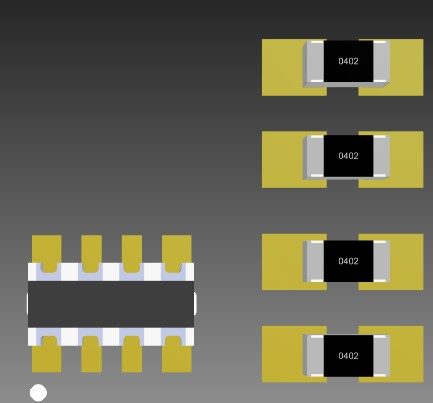
\includegraphics[scale=0.60]{odpor_sit.jpg}
		\caption{Miniaturizace za použití odporových sítí v porovnání s diskrétními odpory.} 
		\label{fig:odpor_sit}
	\end{figure}
	
	\subsection{USB} % Navrh plosnaku, USB C ochrana, popis USB C konektoru
	\label{USB}
	Jako uživatelské rozhraní bylo zvoleno rozhraní USB s konektorem typu USB C. Konkrétně byla použita specifikace USB 2.0 High Speed. Tato specifikace umožňuje komunikovat s maximální přenosovou rychlostí 480 Mbit/s. Vzhledem k maximální vyčítací rychlosti z detektoru Timepix 2, která je dle \ref{Technicka specifikace} 100 Mbit/s, je použití této konkrétní specifikace USB dostačující. 
	\subsubsection{Konektor}
	Konektor byl použit typu USB C. Jednou z výhod konektoru USB C je symetrické zapojení pinů na konektoru. Díky této vlastnosti může uživatel konektor zapojit do vyčítacího rozhraní s libovolnou orientací. Symetrické zapojení signálů na USB C konektoru je možné vidět na obrázku \ref{fig:USBC_full}. K detekci orientace zapojení konektoru, slouží signály označené jako CC1 a CC2. Další funkcí těchto signálů je, že pomocí nich je možné nastavit konkrétní velikost proudu dodávaného do zařízení. Tyto signály jsou přes elektrostatickou ochranu z obrázku \ref{fig:USBC_full} připojeny do mikrokontroléru. 
	\begin{figure}[h!]
		\centering
		\captionsetup{justification=centering}
		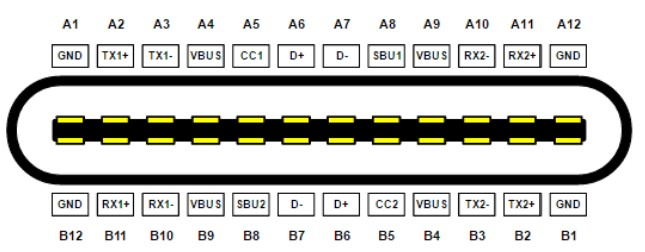
\includegraphics[scale=0.50]{USBC_full.jpg}
		\caption{Schematické rozložení konektoru USB C.} 
		\label{fig:USBC_full}
	\end{figure} 

	\subsubsection{Zapojení}
	Vzhledem k použité specifikaci USB 2.0, je možné některé piny ze zapojení konektoru \ref{fig:USBC_full} nechat nezapojené. Konkrétně jsou to piny s označením TXxx a RXxx, tyto piny slouží pro přenos vysokorychlostní komunikace z USB standartu 3.0 a vyšší. Celkové zapojení použitého konektoru a potřebných elektro statických ochran je možné vidět na obrázku \ref{fig:USBC_zapojeni}. Pro elektrostatickou ochranu diferenciálních datových párů D+ a D- byla použita součástka ECMF02-2AMX6. Dalším prvkem pro ochranu USB signálů a napájení, byla použita součástka TCPP01-M12. Tato součástka zajišťuje ochranu před předpětím na napájecím napětí VBUS. Dále zajišťuje ochranu pinů CC před případných zkratem s napájecím napětí. Odporovým děličem ze zapojení \ref{fig:USBC_zapojeni}, který je tvořený odpory R34 a R36, je možné nastavit maximální hodnotu napájecího napětí, které bude dodáváno na výstupu pinu VBUS USB C konektoru. V této práci je nastaveno maximální napájecí napětí na +6 V. V případě překročení této nastavené úrovně dojde pomocí externího tranzistoru Q1, k odpojení napájecího napětí zařízení. Jedinou částí vyčítacího rozhraní, ke které bude mít uživatel fyzický přístup je právě USB C konektor, proto bylo zvoleno zapojení ochrany, v podobě paralelního zapojení odporu R37 a kondenzátoru 56, na stínění konektoru USB C. 
	\begin{figure}[h!]
		\centering
		\captionsetup{justification=centering}
		%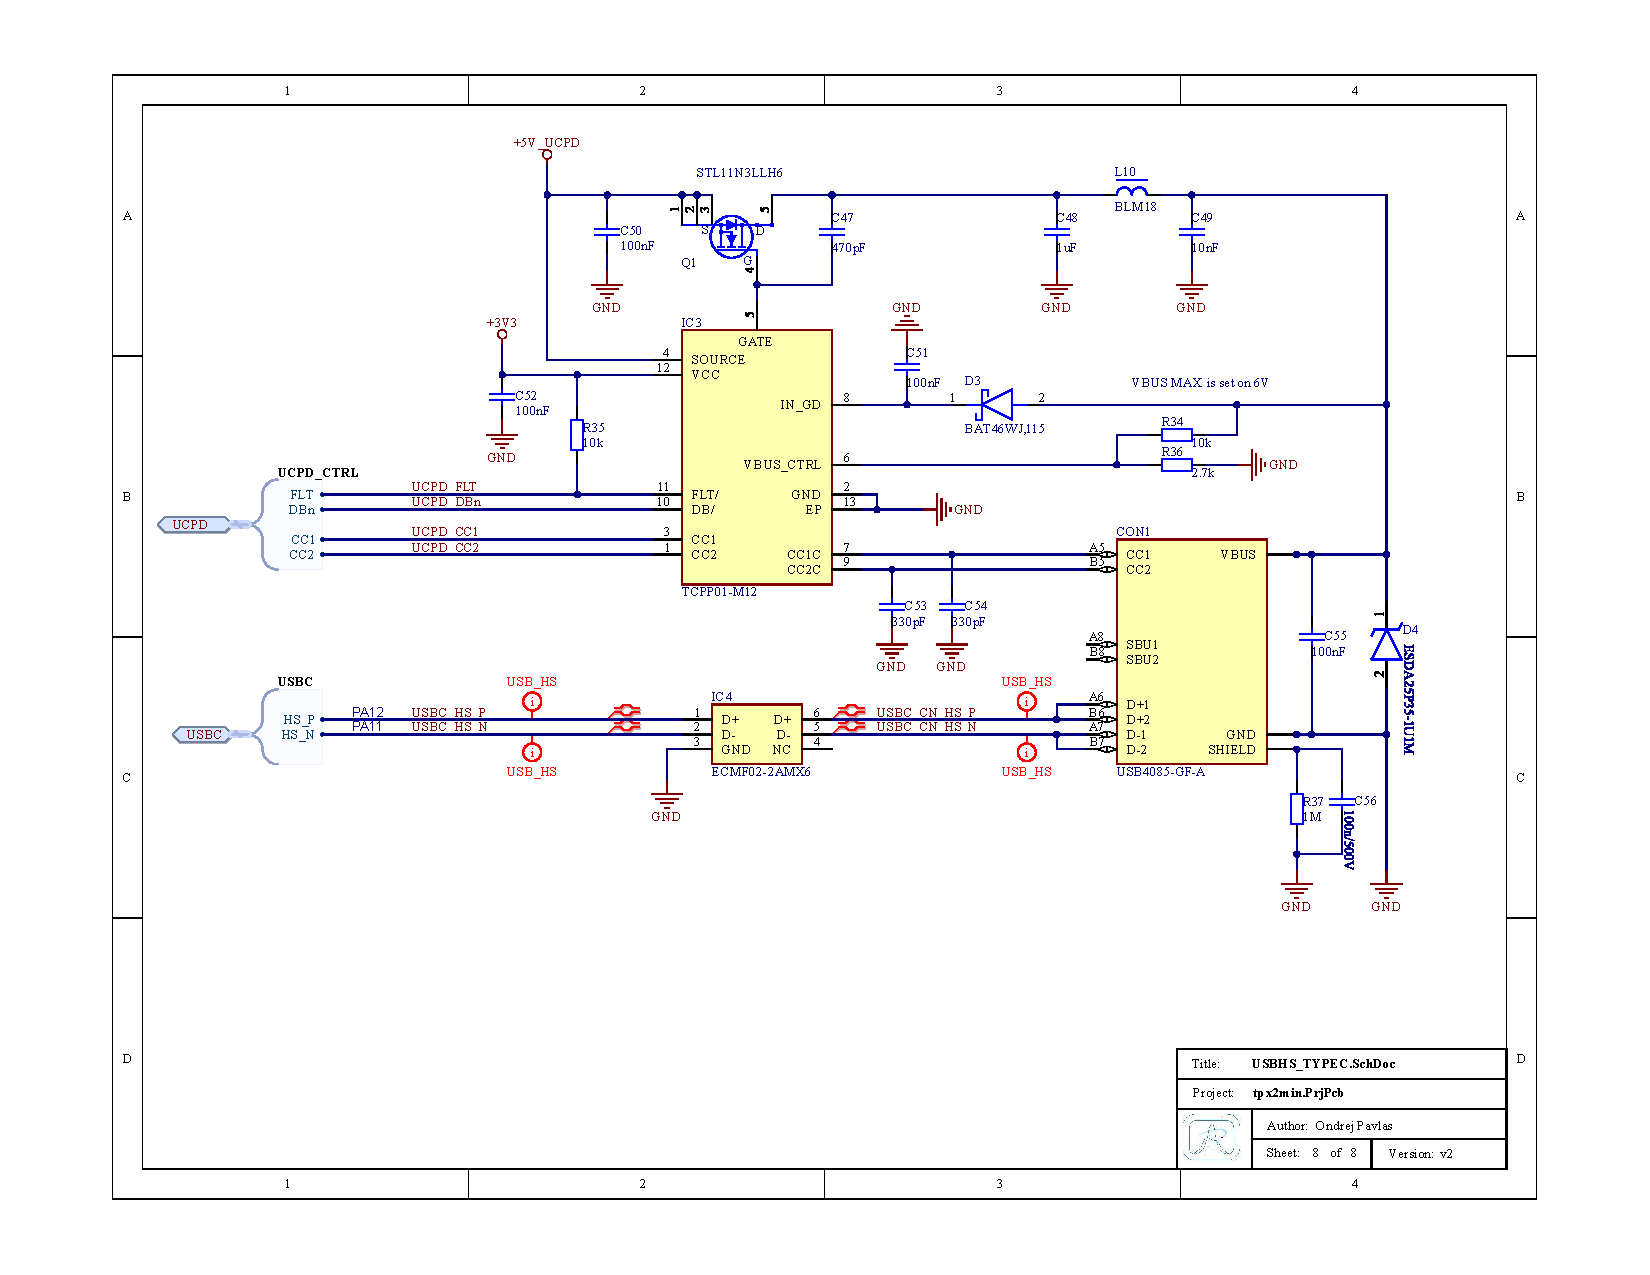
\includepdf[scale=0.7]{usbc.pdf}
		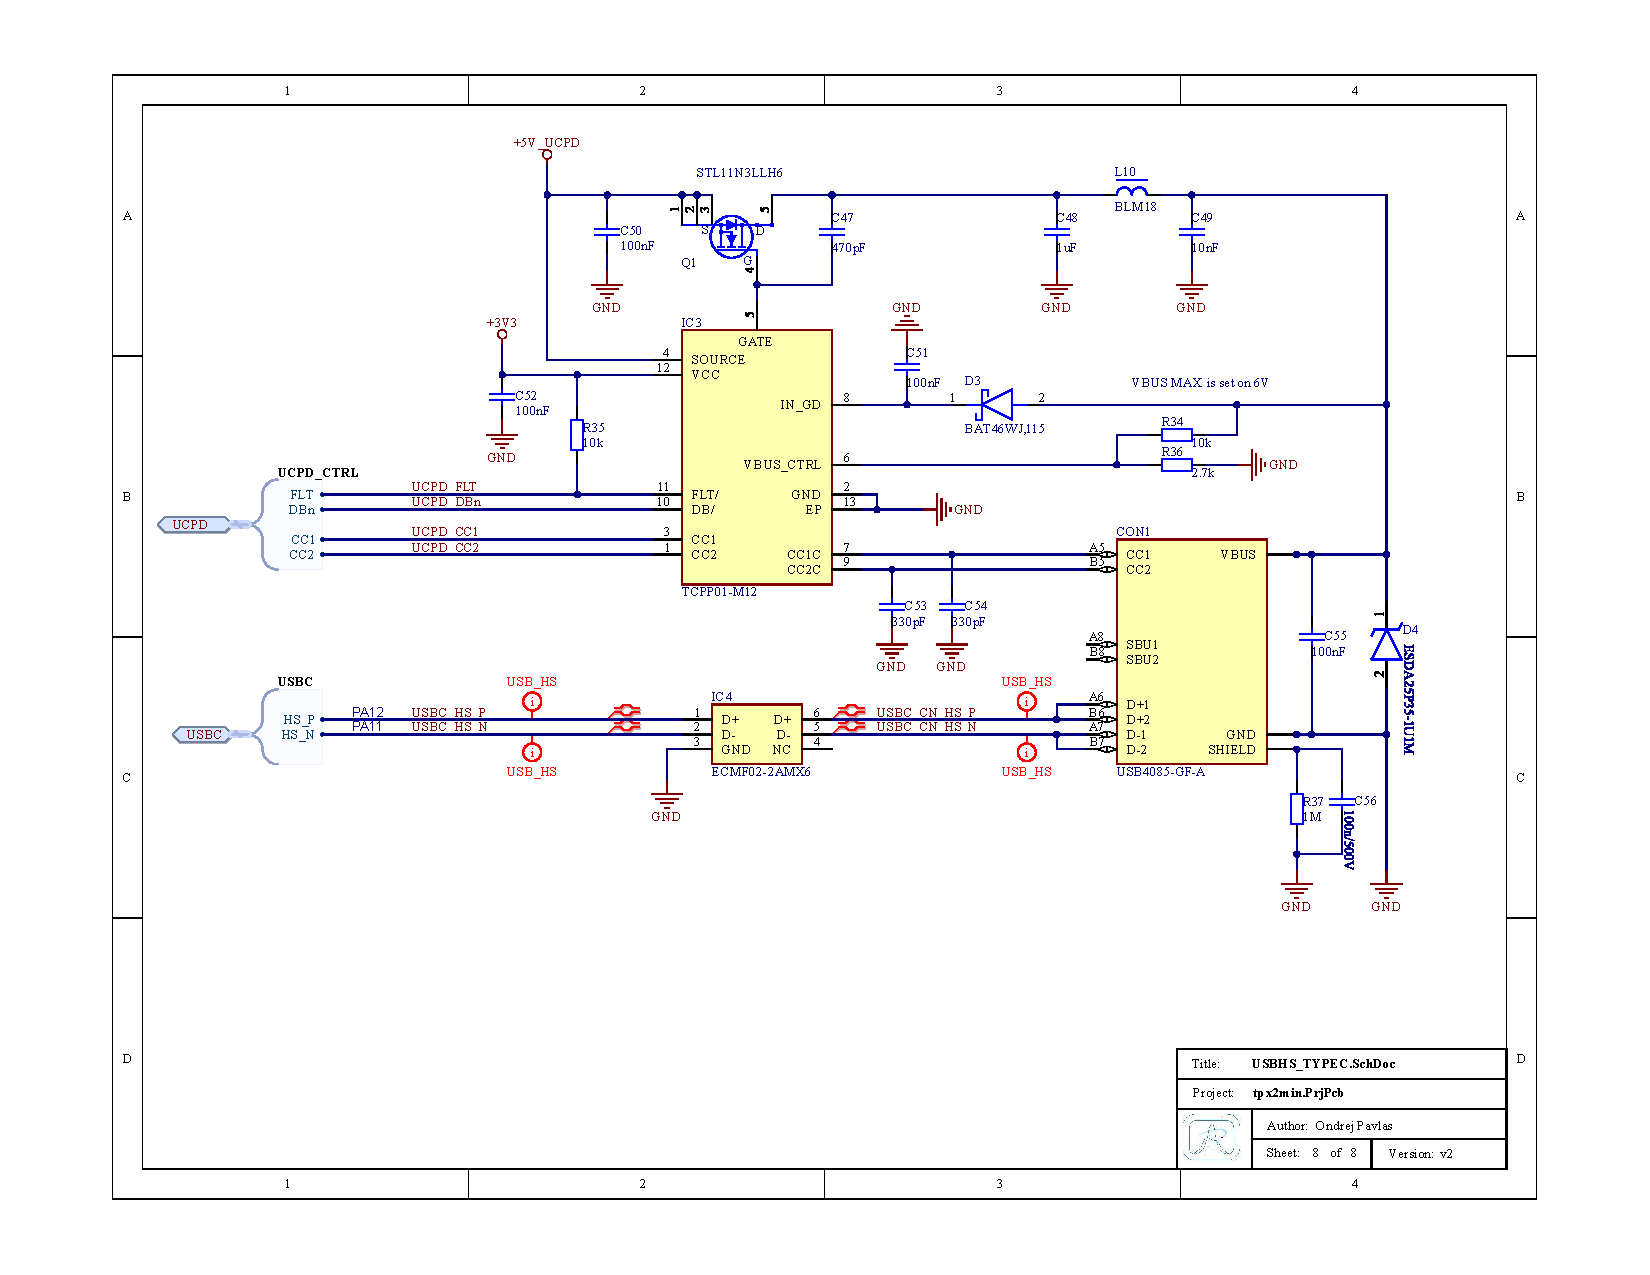
\includegraphics[scale=0.60]{usbc.pdf}
		\caption{Schematické zapojení periférie USB.} 
		\label{fig:USBC_zapojeni}
	\end{figure} 
	
	\subsubsection{PCB}
	Jak bylo zmíněno v předchozí části, maximální komunikační rychlost specifikace USB 2.0 High Speed je 480 Mbit/s. Návrh PCB musel pro část USB musel odpovídat požadavkům pro návrh PCB pro vysokorychlostní komunikaci. Délka diferenciálních datových párů D+ a D- byla vůči sobě vykompenzována na vzdálenost 1 mm. Dle technické specifikace USB 2.0 High Speed je doba náběžné ($t_r$), respektive sestupné ($t_f$) hrany 500 ps. Časové zpoždění ($\Delta t$) mezi datovými páry D+ a D- by mělo být výrazně menší, než doba ($t_r$), respektive ($t_f$). Pokud zvolíme maximální časové zpoždění mezi páry D+ a D- na hodnotu 25 ps, při uvažované hodnotě zpoždění 0.1 ns/cm na plošném spoji, je nutné diferenciální signály vykompenzovat, tak aby maximální rozdíl délek vodičů diferenciálních párů, nebyl větší než 2.5 mm. Jak bylo již zmíněno, v uvedené práci došlo ke délky diferenciálních párů na 1 mm. Tedy časové zpoždění mezi páry, nebude větší než 10 ps.
	\par Diferenciální páry D+ a D- byly po PCB vedeny ve vrchní a spodní vrstvě plošného spoje. Dle celkové skladby PCB základní desky z tabulky \ref{tab:pcb_vrstvy} odpovídá, že sousedící vrstva, respektive vrstvy pod vrchní a spodní vrstvou je vždy souvislou zemní plochou. Z celkové skladby PCB z obrázku \ref{fig:PCB_mother_stackup}, byly výrobcem PCB dodané parametry pro fyzické rozměry diferenciálních vodičů, aby bylo možné dodržení impedančního přizpůsobení $100 \Omega$. Realizaci vedení signálů D+ a D- na desce plošných spojů je možné vidět na obrázku \ref{fig:usb_layout}
	
	\begin{figure}[h!]
		\begin{subfigure}{0.5\textwidth}
			\centering
			\captionsetup{justification=centering}
			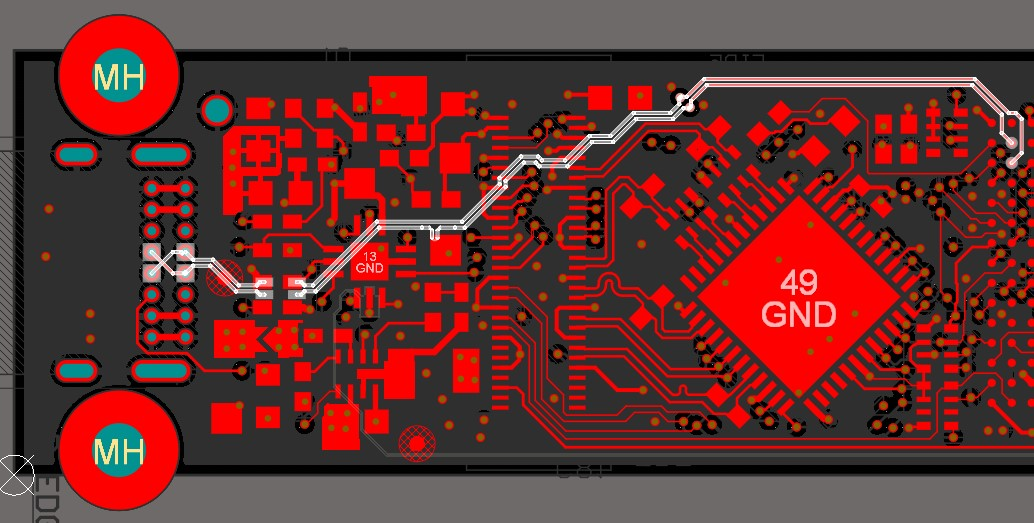
\includegraphics[scale=0.33]{usb_hs_top.jpg}
			\caption{Signály USB, D+ a D-, vrchní vrstva PCB.} 
			\label{fig:usb_top}
		\end{subfigure} \hfill
		\begin{subfigure}{0.5\textwidth}
			\centering
			\captionsetup{justification=centering}
			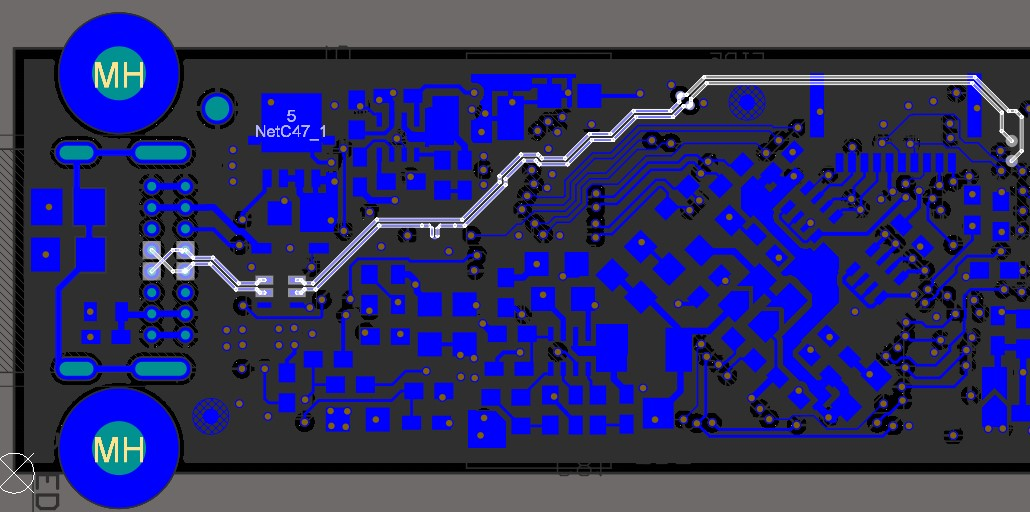
\includegraphics[scale=0.33]{usb_hs_bot.jpg}
			\caption{Signály USB, D+ a D-, spodní vrstva PCB.} 
			\label{fig:usb_bot}
		\end{subfigure}
		\caption{Vedení diferenciálních datových páru periférie USB.}
		\label{fig:usb_layout}
	\end{figure} 


\section{Deska s Timepix 2}
	\label{Deska s Timepix2}
	Druhou deskou plošných spojů v této práci je deska s detektorem Timepix 2 z blokového zapojení z obrázku konceptu řešení \ref{fig:navrh_reseni}. Tato deska je propojena se základní deskou za pomocí 60 pinového konektoru ze série DF40 od společnosti Hirose Electric Group. Rozložení signálů na konektoru lze najít v příloze zapojení celé práce \ref{Priloha základní deska}, nebo v části textu \ref{konektor}.
	
	\par Deska s Timepix 2 je navržena na šestivrstvém plošném spoji. Skladba plošného spoje je analogická se skladbou PCB pro základní desku, viz. obrázek \ref{fig:PCB_mother_stackup} a tabulka \ref{tab:pcb_vrstvy}. Rozměry desky s detektorem Timepix 2 jsou poté 53 x 17 mm. 
\subsection{Timepix 2}	% 
	Nejdůležitější částí celé práce je samotný pixelový detektor radiace Timepix 2. Specifikace pixelového detektoru Timepix 2 byly popsány v části \ref{Technicka specifikace}. Nadále bude popsána realizace pro splnění všech specifikacích nutných pro provoz pixelového detektoru Timepix 2.
	\subsubsection{Napájení}	% popsat jak se bere z konektoru plus prepinani pro chipID
	Dle \ref{tab:tpx2_napajeni} je pro korektní provoz Timepix 2 zapotřebí celkem třech napájecí napětí. Napájecí napětí pro vstupní/výstupní bránu detektoru Timepix 2 označovanou jako VDDIO s velikostí napájecího napětí +2.5 V se generuje na základní desce. Tedy toto napájení je vedeno přes konektor ze základní desky a je poté na desce s detektorem přivedeno k příslušným pinům Timepix 2.
	\par Napájení pro digitální a analogovou část Timepix 2 se generuje přímo na této desce. Z označení z tabulky \ref{tab:tpx2_napajeni} se jedná o napájení VDD a VDDA. Zapojení regulátorů pro tyto napájecí napětí můžete vidět na obrázku \ref{fig:tpx_pwr}. Pro napájení digitální části Timepix 2 byl použit stejný spínaný regulátor, jako na základní desce \ref{fig:mp2333h}. Pro napájení analogové části byl použit lineární stabilizátor od společnosti Texas Instruments TPS7A94, který ze vstupních +2.5 V reguluje napětí na výstupních +1.2 V. Oba uvedené regulátory jsou řízené z mikrokontroléru, který je umístěn na základní desce \ref{zakladni deska}.
	\begin{figure}[h!]
		\centering
		\captionsetup{justification=centering}
		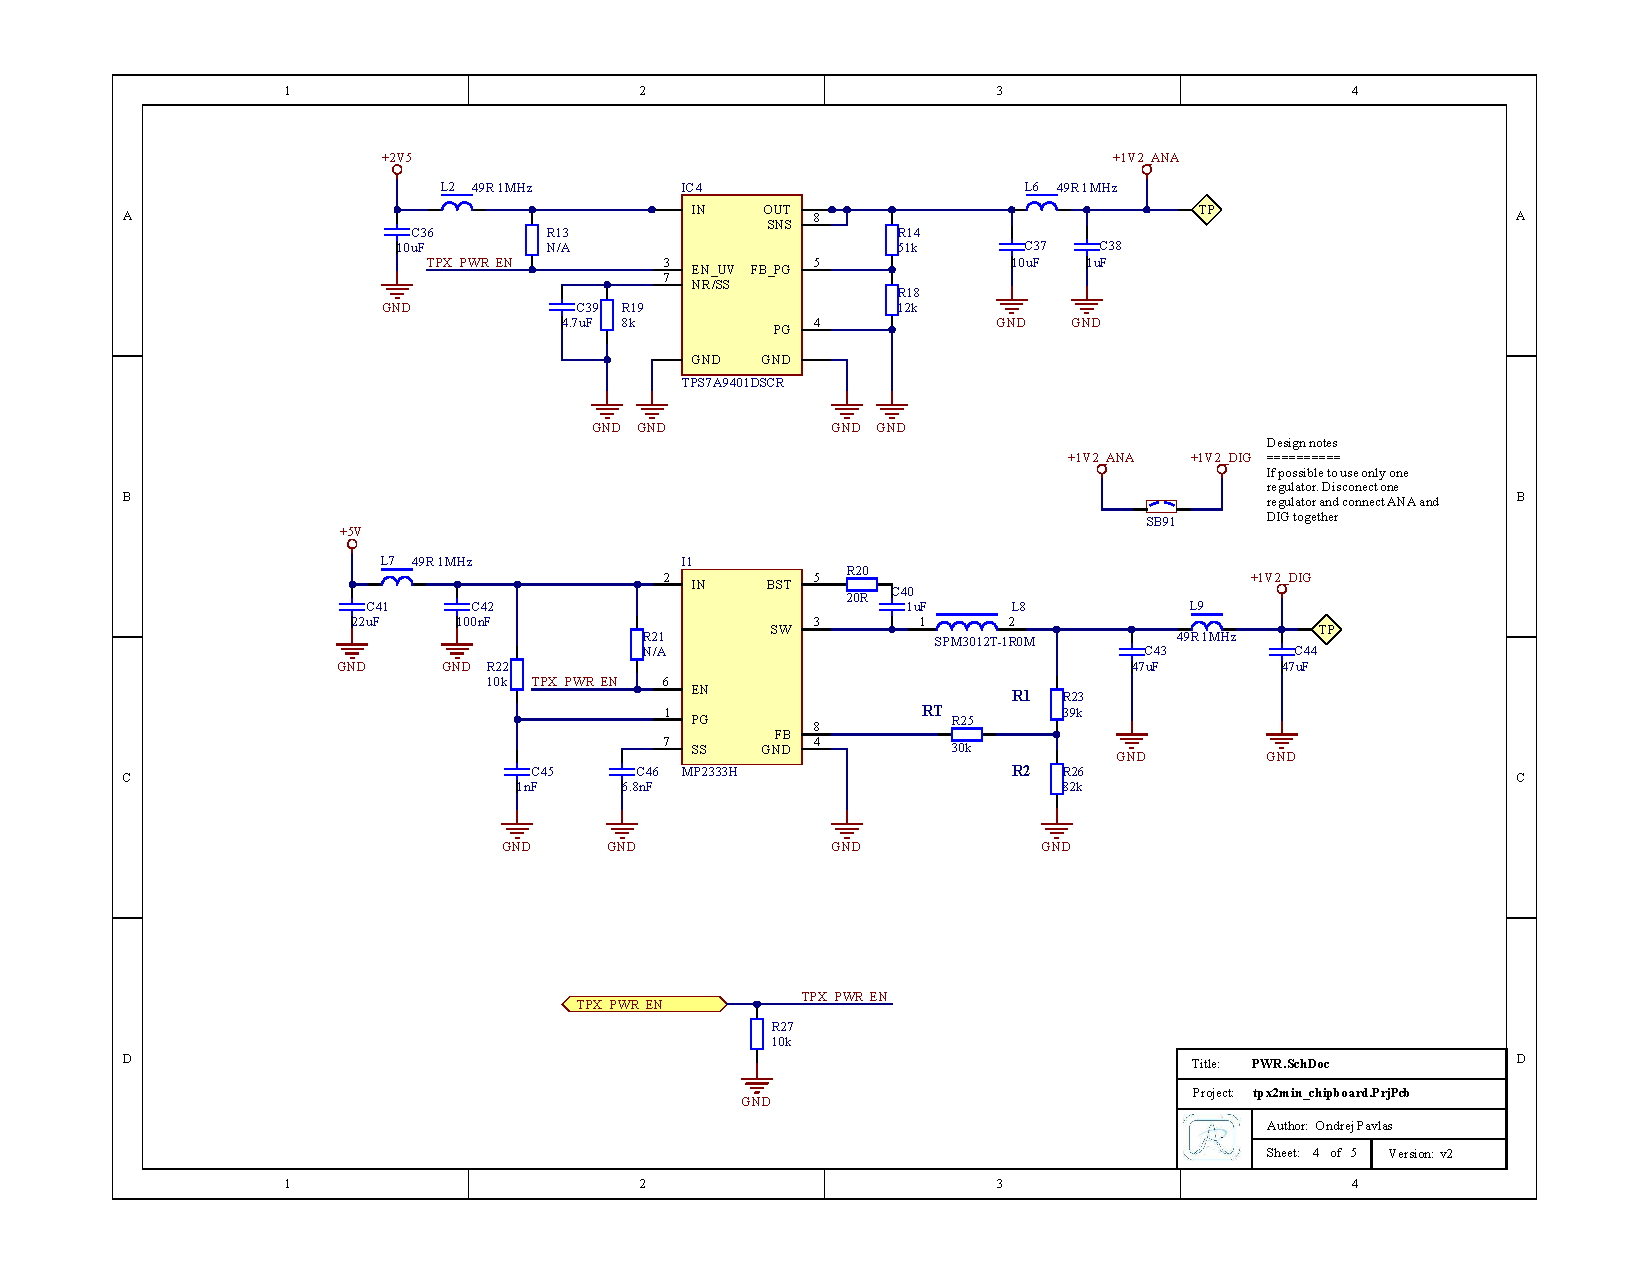
\includegraphics[scale=0.60]{tpx_pwr.pdf}
		\caption{Realizace analogového a digitální napájení detektoru Timepix 2.} 
		\label{fig:tpx_pwr}
	\end{figure} 
	\subsubsection{Rozhraní pro připojení Timepix 2}	% wirebondovaci plosky, HV zdroj
	Pro připojení Timepix 2 k desce plošných spojů byly použity wirebondovcí plošky na vrchní straně detektoru Timepix 2, které je možné vidět na spodní straně obrázku \ref{fig:tpx2_floorplan}. Celekm bylo u této práce realizováno propojení 128 wirebondovacích plošek z Timepix 2 na chipboardovou desku. Plošky na straně PCB jsou umístěny ve dvou řadách. Rozteč mezi jednotlivými plošky je 0.2mm, šířka plošek je poté 0.1 mm. V pravé části obrázku \ref{fig:tpx_wire} můžete vidět plošku pro připojení vysokého napětí na senzorovou vrstvu Timepix 2. Toto vysoké napětí slouží k vytvoření vyprázdněné oblasti v senzorové vrstvě, více o významu připojeného vysokého napětí bylo popsáno v části \ref{kap:2.1}. 
	\begin{figure}[h!]
		\centering
		\captionsetup{justification=centering}
		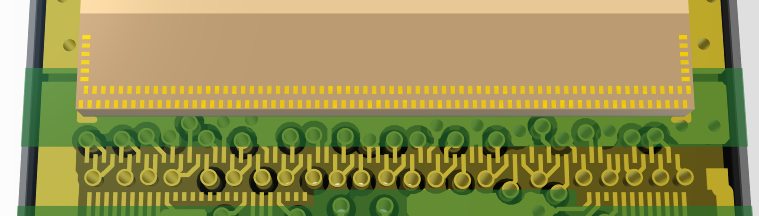
\includegraphics[scale=0.60]{tpx_wire.png}
		\caption{Rozložení pinů pro připojení Timepix 2 k desce plošných spojů.} 
		\label{fig:tpx_wire}
	\end{figure} 
	\subsection{Vysokonapěťový zdroj}	% MAX1932 zapojeni vysvetleni
	\label{VN zdroj}
	Vysokonapěťový zdroj pro tuto práci byl realizován za použití součástky od společnosti Analog Devices, konkrétně byla použita součástka MAX1932 \cite{MAX1932}. Jedná se o vysokonapěťový zdroj s nastavitelnou úrovní výstupního napětí 30 - 148 V. Úroveň výstupního napětí se nastavuje pomocí SPI komunikace v uvedeném rozsahu s rozlišením 256 hodnot. Schematické zapojení vysokonapěťového zdroje je možné vidět na obrázku \ref{fig:hv}. Hodnota velikosti výstupního napětí lze nastavit pomocí odporů ve zpětné vazbě regulátoru ze zapojení \ref{fig:hv} a to dle následujících rovnic \ref{eq:R5} a \ref{eq:R6}. 
	\begin{equation}
		R5 = (V_{OUT01} - V_{OUTFF})\cdot (R6/1.25V)
		\label{eq:R5}
	\end{equation}

	\begin{equation}
		R8 = \frac{1.25V \cdot R5}{V_{OUTFF}}
		\label{eq:R6}
	\end{equation}
	Kde $V_{OUT01}$ je maximální nastavené výstupní napětí a $V_{OUTFF}$ je minimální nastavené napětí. 
	\begin{figure}[h!]
		\centering
		\captionsetup{justification=centering}
		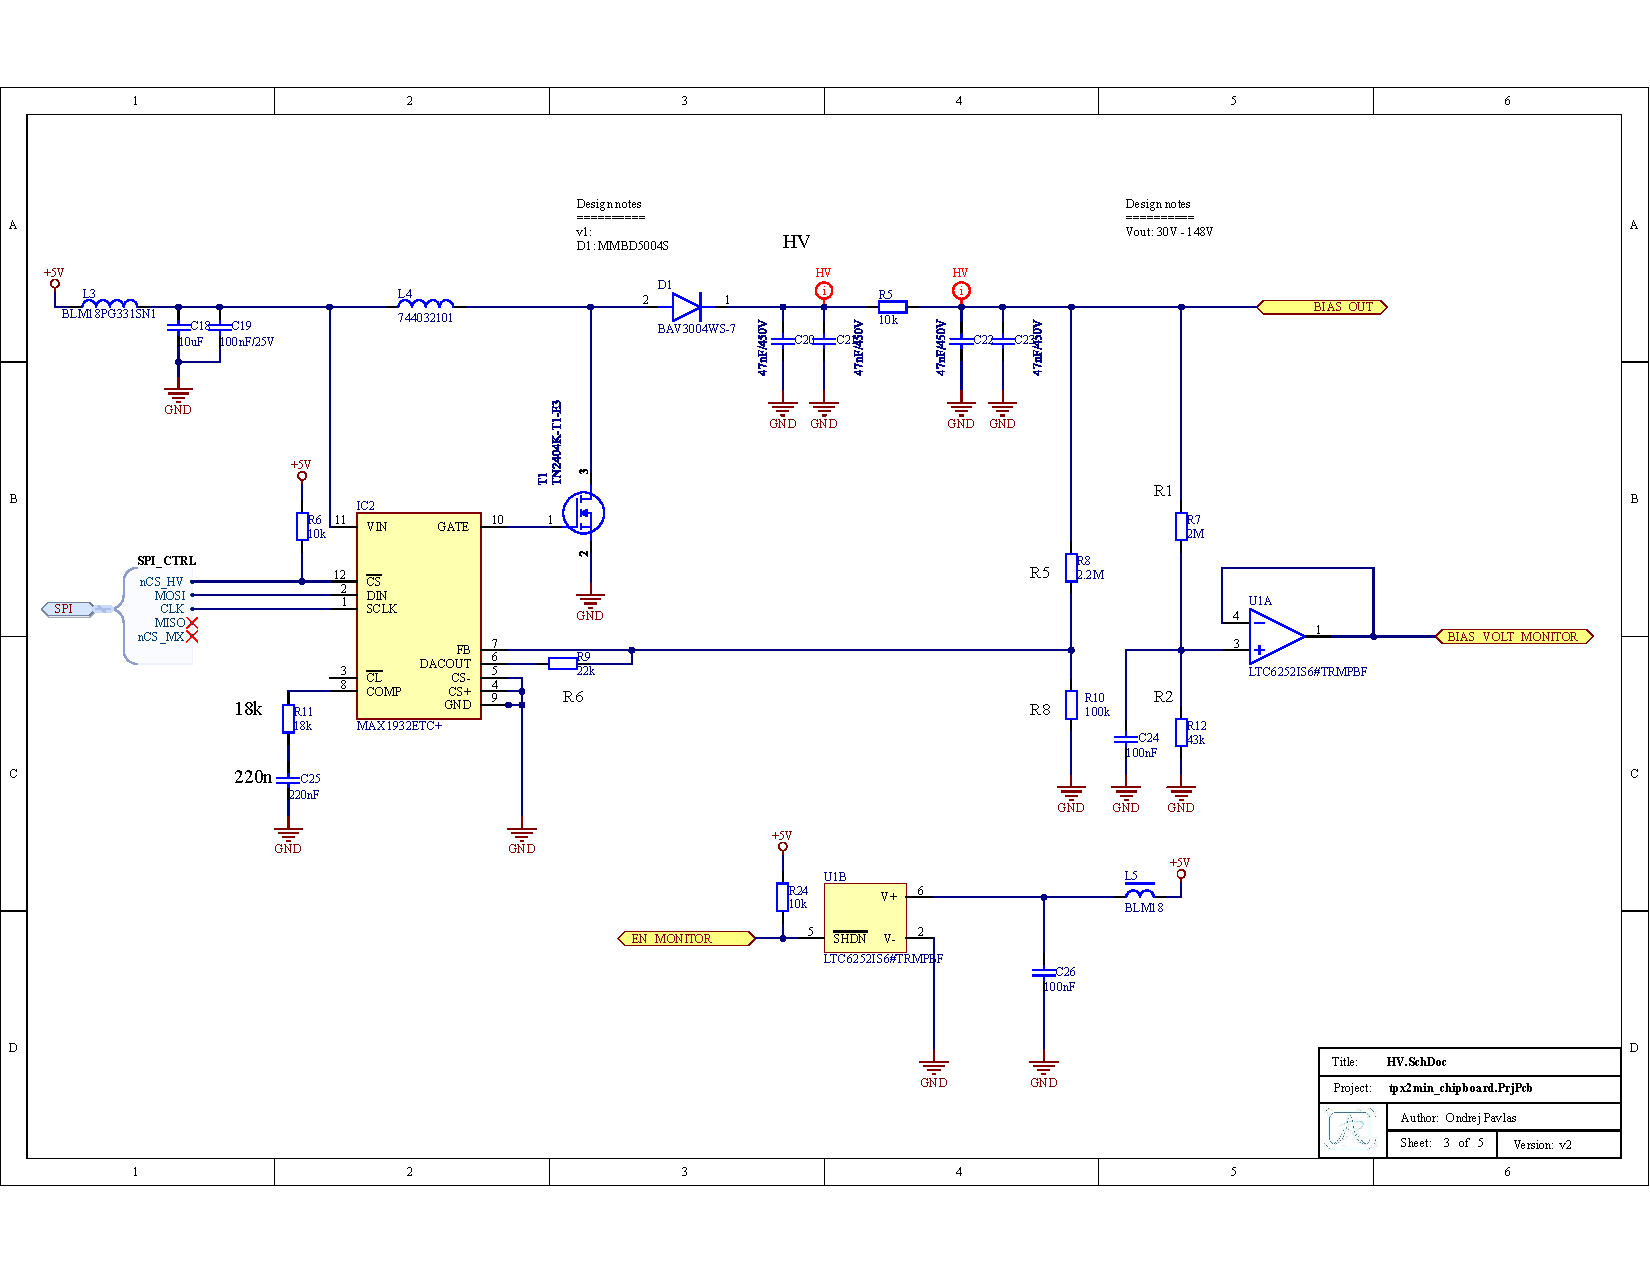
\includegraphics[scale=0.60]{hv.pdf}
		\caption{Schematické zapojení vysokonapěťového zdroje MAX1932.} 
		\label{fig:hv}
	\end{figure} 
	\subsubsection{Měření vysokého napětí} % napetovy sledovac plus konfigurace AD v STM32
	Pro měření vysokého napětí byl použit operační zesilovač v zapojení napěťového sledovače z obrázku \ref{fig:hv} v pravé části. Přesněji byl použit operační zesilovač od společnosti Analog Devices LTC6262 \cite{LTC6252}. Výstup operačního zesilovače je poté připojen na vstupní pin mikrokontroléru, který je nakonfigurován jako analogový vstup. Pomocí interního 14-bitového AD převodníku mikrokontroléru je převedena analogová hodnota odpovídající hodnotě vysokého napětí do digitální formy. Následně je tato hodnota dostupná pro pro další programové zpracování. 

	\subsection{Měření teploty}	% proces nastaveni senzoru atd
	\label{Mereni teploty}
	Pro měření teploty na desce s detektorem Timepix 2 byl použit senzor TMP100 \cite{TMP100} od společnosti Texas Instruments. Jedná se o senzor disponující 12 bitovým rozlišením s přesností $\pm 1^{\circ} C$ v rozsahu teplot od $-55^{\circ}C$ do $125^{\circ}C$. Komunikace se senzorem a vyčítaní dat probíhá pomocí I2C sběrnice. Zapojení senzoru je vidět na obrázku \ref{fig:tmp100}. Fyzická adresa senzoru pro I2C komunikaci, je nastavena pomocí pinů ADD0 a ADD1 na hexadecimální hodnotu 0x48.
	\begin{figure}[h!]
		\centering
		\captionsetup{justification=centering}
		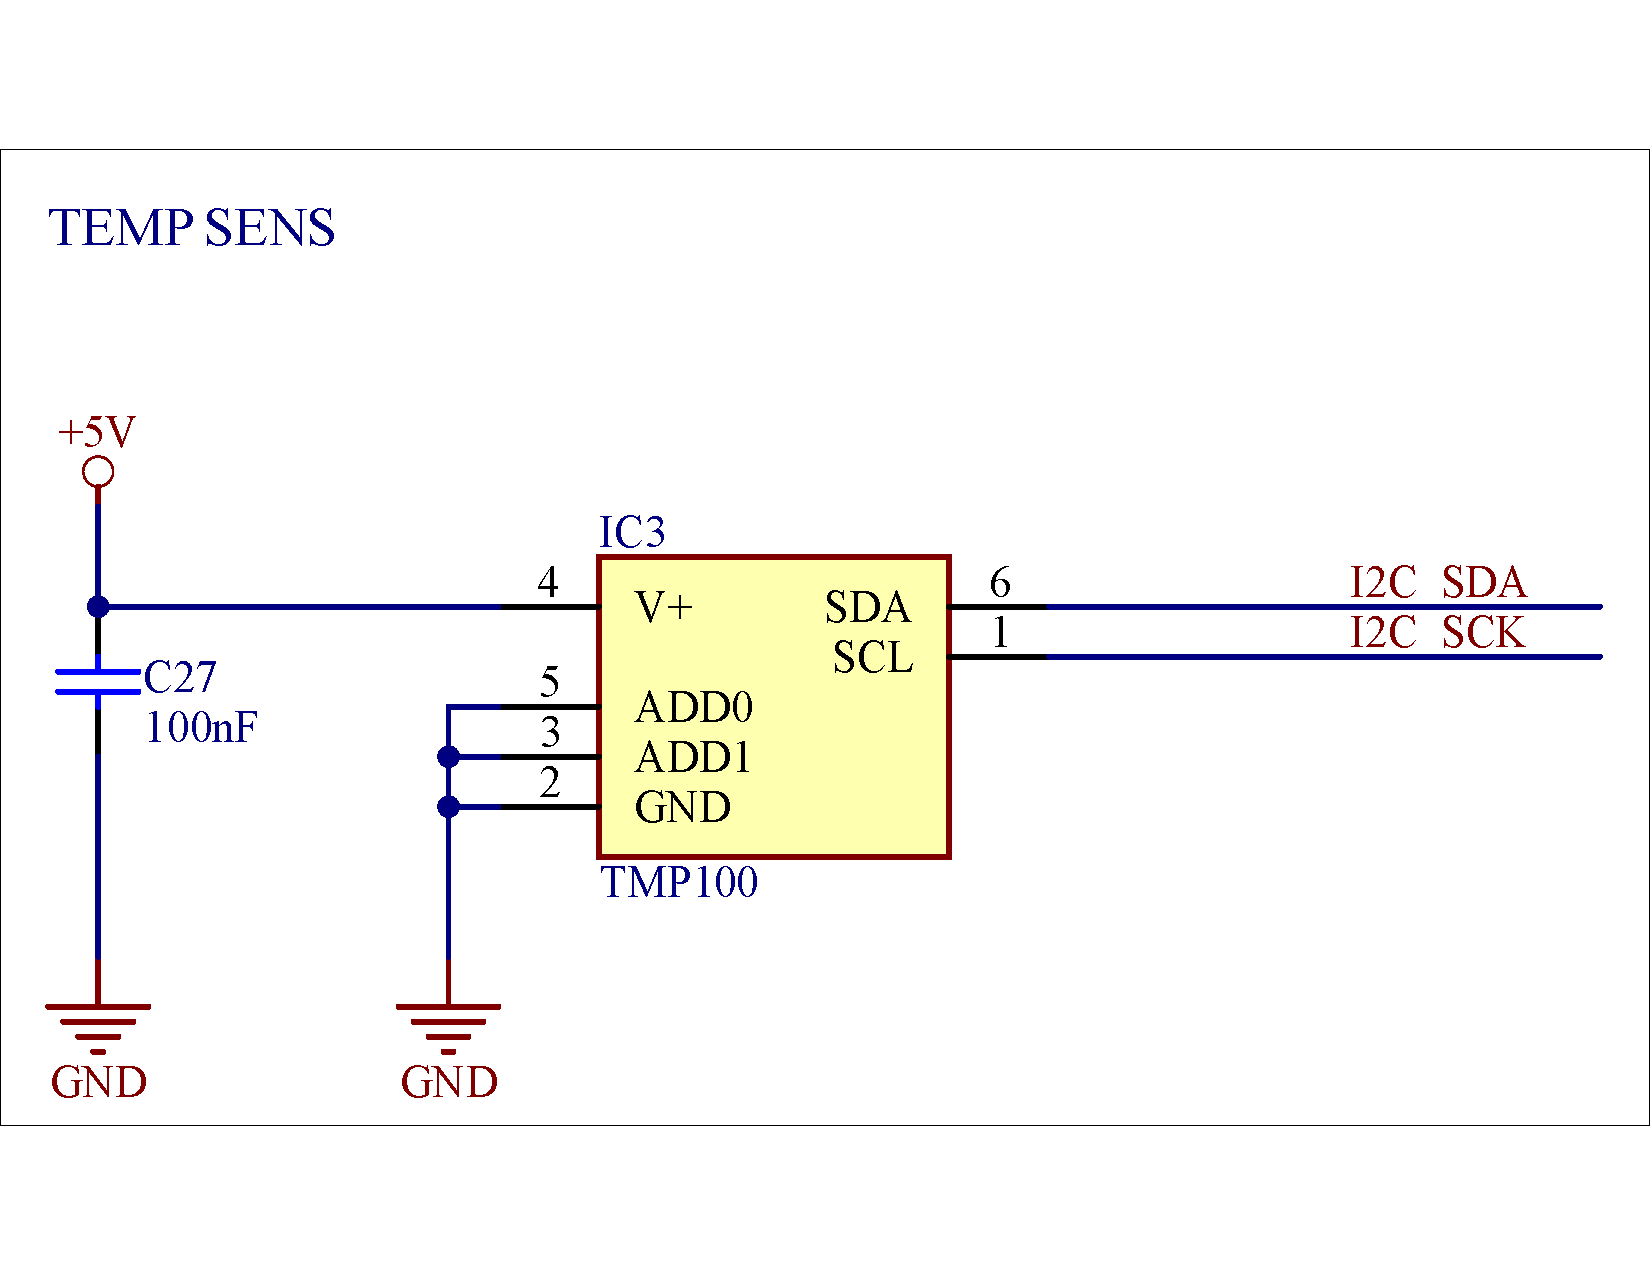
\includegraphics[scale=0.30]{temp.pdf}
		\caption{Zapojení teplotního senzoru TMP100.} 
		\label{fig:tmp100}
	\end{figure} 
	\subsection{Konektor}	% popis konektoru, zarazeni zmneni mezi piny
	\label{konektor}
	Rozložení konektoru mezi základní deskou \ref{zakladni deska} a deskou s Timepix 2 \ref{Deska s Timepix2} je vidět na obrázku \ref{fig:konektor}. Pro propojení desek byl použit konektor DF40C-60DP-0.4V(51) od společnosti Hihorse Connector. Rozteč jednotlivých kontaktů konektoru je 0.4 mm. Tento konektor byl použit ve variantě, kdy celková výška mezi základní deskou a deskou s Timepix 2 je 2.5 mm. Výhodou tohoto konektoru je možnost volby výšky konektoru, dle výběru, nabízeného výrobcem. Na desce s Timepix 2 jsou ze záladní desky dostupné celkem 3 napájecí úrovně a to +2.5 V, +3.3 V a +5 V. Rozložení vysokorychlostních diferenciálních párů na konektoru bylo pro každý diferenciální pár odděleno zapojením země mezi jednotlivé páry, jak lze vidět ze zapojení \ref{fig:konektor} v pravé části. Toto zapojení bylo navrhnuto s ohledem na minimalizaci přeslechů mezi jednotlivými diferenciálními páry.
	\begin{figure}[h!]
		\centering
		\captionsetup{justification=centering}
		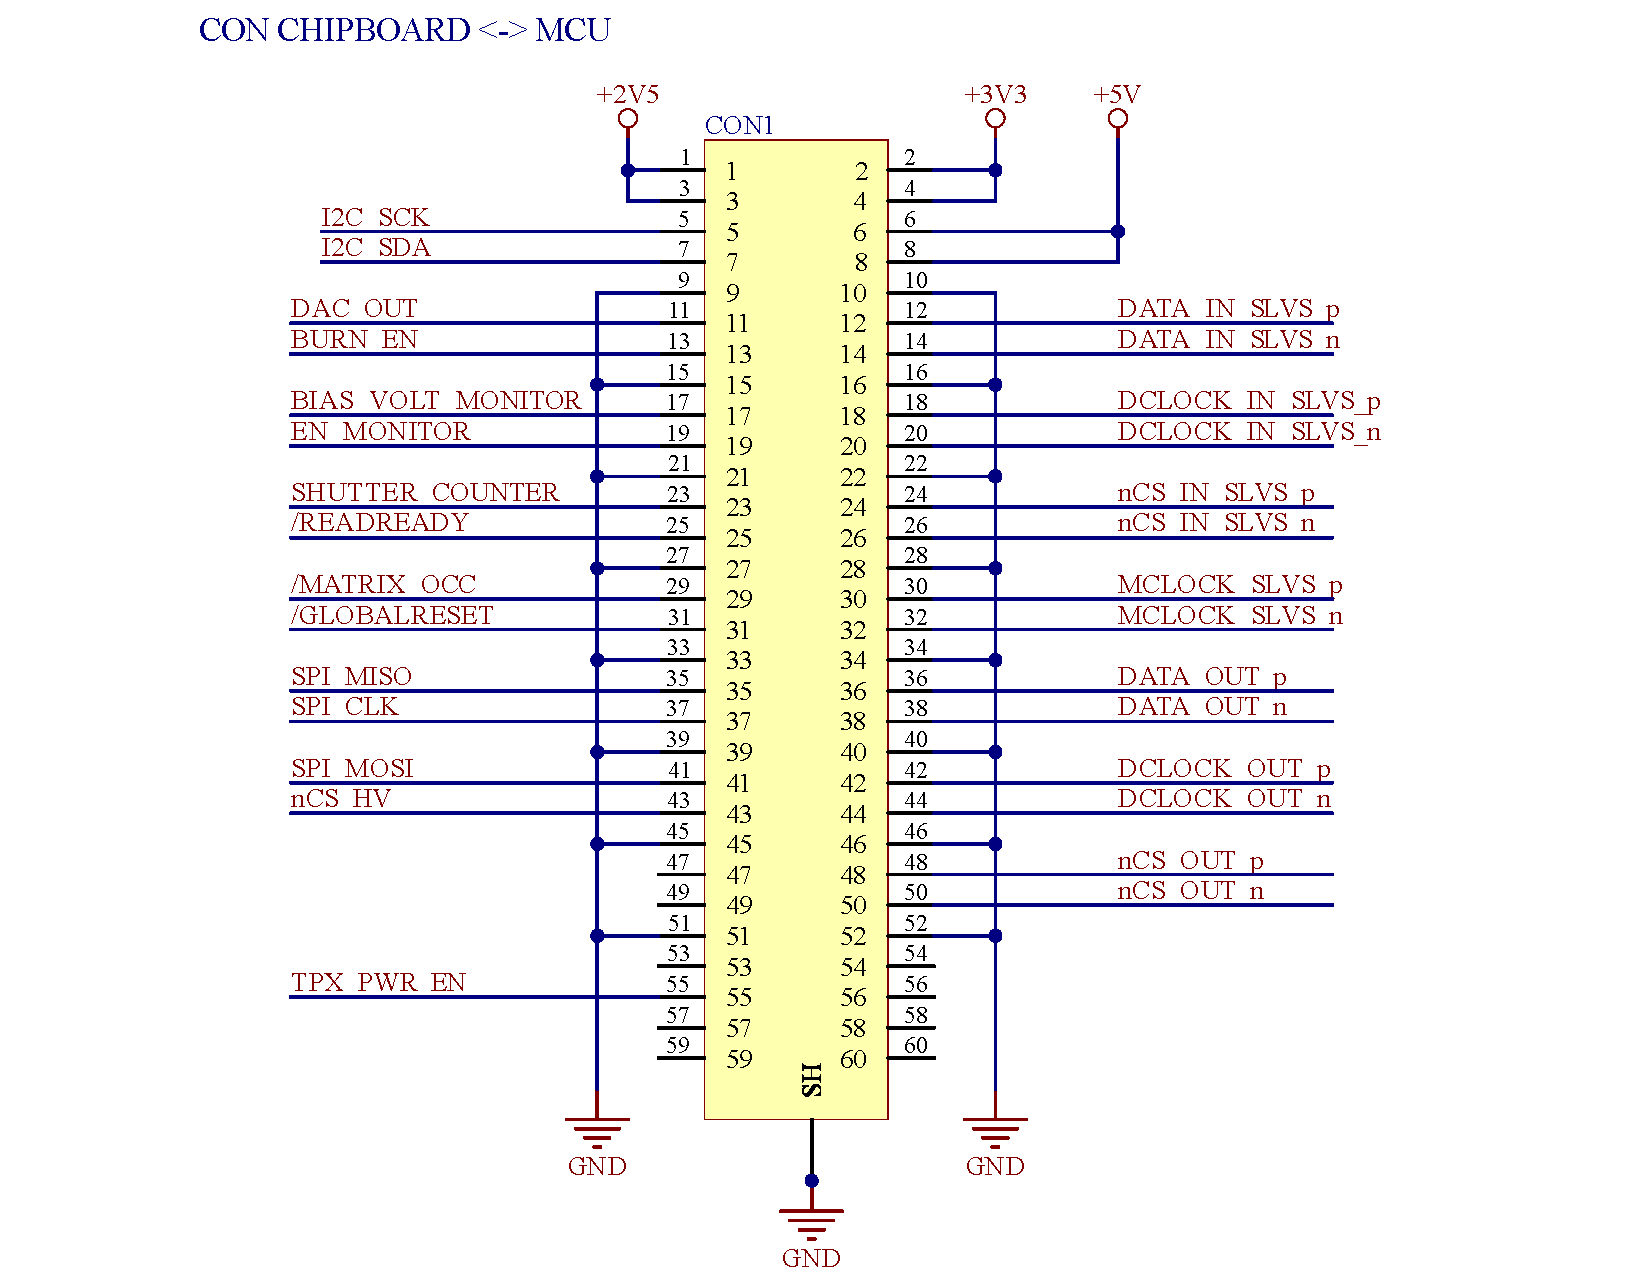
\includegraphics[scale=0.40]{conn.pdf}
		\caption{Zapojení konektoru mezi základní deskou \ref{zakladni deska} a deskou s Timepix 2 \ref{Deska s Timepix2}.} 
		\label{fig:konektor}
	\end{figure} 
	
\section{Mechanika}
	Mechanickým řešením byla zvolena výroba hliníkové krabičky. Hliník byl vybrán díky svým teplo vodivým vlastnostem, váhou a dobrou obrobitelností. Navržená mechanická krabička byla vyfrézovaná na CNC zařízení. Na výsledný povrch mechanické krabičky byl nanesen černý elox s potiskem loga Ústavu Technické a Experimentální Fyziky ČVUT, kde celá tato práce byla realizována. Výslednou mechanickou krabičku je možné vidět na obrázku \ref{fig:mechanika}. Na obrázku můžete vidět nalepenou teplo vodivou pásku která slouží pro zlepšení odvodu tepla z detektoru Timepix 2 do celého objemu navržené mechanické krabičky. Na vrchní straně krabičky je možné vidět posuvné okénko, jež slouží po složení celé mechaniky k zakrytí části s detektorem Timepix 2, aby při manipulaci s rozhraním nedošlo k poškození detektoru. Při měření je možné toto výsuvné okénko nastavit do pozice otevřeno. Rozměry mechaniky jsou 73.4 x 22 x 13.5 mm. 
	%TODO krabika fota
	\begin{figure}[h!]
		\centering
		\captionsetup{justification=centering}
		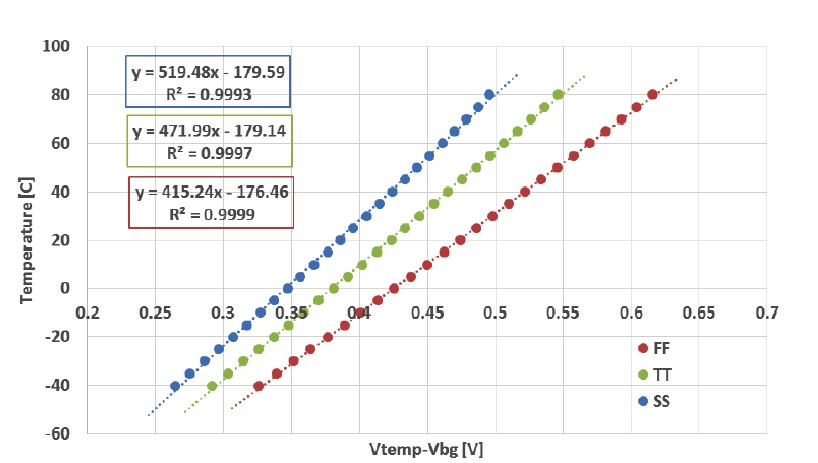
\includegraphics[scale=0.60]{tpx2_temp.jpg}
		\caption{Mechanická krabička navrženého vyčítacího rozhraní.} 
		\label{fig:mechanika}
	\end{figure}

